\section{oosalizer/webalizer.h-Dateireferenz}
\label{webalizer_8h}\index{oosalizer/webalizer.h@{oosalizer/webalizer.h}}


Dieser Graph zeigt, welche Datei direkt oder indirekt diese Datei enth\"{a}lt:\begin{figure}[H]
\begin{center}
\leavevmode
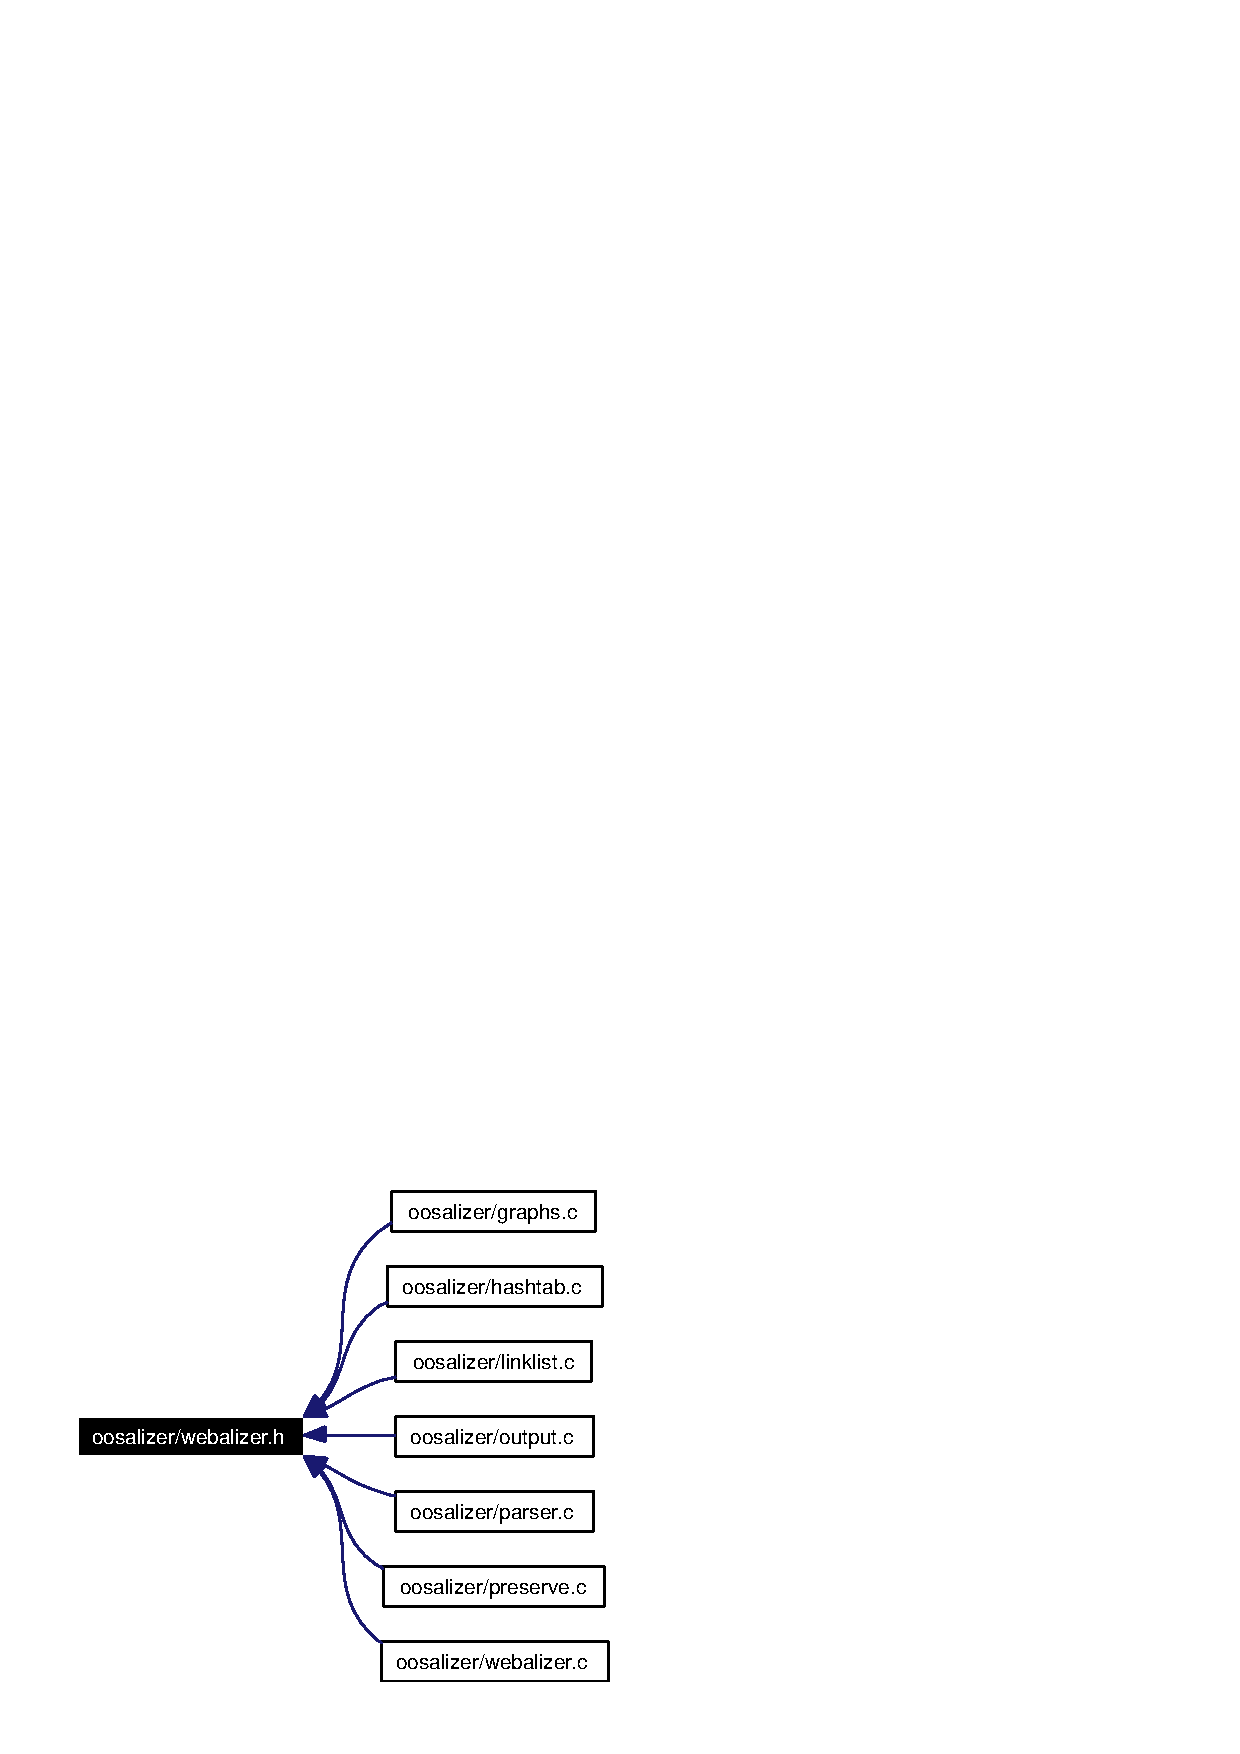
\includegraphics[width=146pt]{webalizer_8h__dep__incl}
\end{center}
\end{figure}
\subsection*{Datenstrukturen}
\begin{CompactItemize}
\item 
struct {\bf response\_\-code}
\item 
struct {\bf response\_\-url}
\item 
struct {\bf responsetmp\_\-url}
\item 
struct {\bf country\_\-code}
\item 
struct {\bf log\_\-struct}
\end{CompactItemize}
\subsection*{Makrodefinitionen}
\begin{CompactItemize}
\item 
\#define {\bf PCENT}(val, max)~((val)?((double)val/(double)max)$\ast$100.0 : 0.0)
\item 
\#define {\bf IDX\_\-2C}(c1, c2)~(((c1-'a'+1)$<$$<$5)+(c2-'a'+1) )
\item 
\#define {\bf IDX\_\-3C}(c1, c2, c3)~(((c1-'a'+1)$<$$<$10)+((c2-'a'+1)$<$$<$5)+(c3-'a'+1) )
\item 
\#define {\bf IDX\_\-4C}(c1, c2, c3, c4)~(((c1-'a'+1)$<$$<$15)+((c2-'a'+1)$<$$<$10)+((c3-'a'+1)$<$$<$5)+(c4-'a'+1) )
\item 
\#define {\bf MAX}(a, b)~((a) $>$ (b) ? (a) : (b))
\item 
\#define {\bf MAXRESP}~1000
\item 
\#define {\bf INCRESP}~500
\item 
\#define {\bf MAXHASH}~2048
\item 
\#define {\bf BUFSIZE}~4096
\item 
\#define {\bf MAXHOST}~128
\item 
\#define {\bf MAXURL}~2048
\item 
\#define {\bf MAXURLH}~512
\item 
\#define {\bf MAXREF}~2048
\item 
\#define {\bf MAXREFH}~512
\item 
\#define {\bf MAXAGENT}~512
\item 
\#define {\bf MAXCTRY}~48
\item 
\#define {\bf MAXSRCH}~512
\item 
\#define {\bf MAXSRCHH}~128
\item 
\#define {\bf MAXIDENT}~64
\item 
\#define {\bf SLOP\_\-VAL}~3600
\item 
\#define {\bf LOG\_\-CLF}~0
\item 
\#define {\bf LOG\_\-FTP}~1
\item 
\#define {\bf LOG\_\-SQUID}~2
\item 
\#define {\bf RC\_\-CONTINUE}~100
\item 
\#define {\bf RC\_\-SWITCHPROTO}~101
\item 
\#define {\bf RC\_\-OK}~200
\item 
\#define {\bf RC\_\-CREATED}~201
\item 
\#define {\bf RC\_\-ACCEPTED}~202
\item 
\#define {\bf RC\_\-NONAUTHINFO}~203
\item 
\#define {\bf RC\_\-NOCONTENT}~204
\item 
\#define {\bf RC\_\-RESETCONTENT}~205
\item 
\#define {\bf RC\_\-PARTIALCONTENT}~206
\item 
\#define {\bf RC\_\-MULTIPLECHOICES}~300
\item 
\#define {\bf RC\_\-MOVEDPERM}~301
\item 
\#define {\bf RC\_\-MOVEDTEMP}~302
\item 
\#define {\bf RC\_\-SEEOTHER}~303
\item 
\#define {\bf RC\_\-NOMOD}~304
\item 
\#define {\bf RC\_\-USEPROXY}~305
\item 
\#define {\bf RC\_\-MOVEDTEMPORARILY}~307
\item 
\#define {\bf RC\_\-BAD}~400
\item 
\#define {\bf RC\_\-UNAUTH}~401
\item 
\#define {\bf RC\_\-PAYMENTREQ}~402
\item 
\#define {\bf RC\_\-FORBIDDEN}~403
\item 
\#define {\bf RC\_\-NOTFOUND}~404
\item 
\#define {\bf RC\_\-METHODNOTALLOWED}~405
\item 
\#define {\bf RC\_\-NOTACCEPTABLE}~406
\item 
\#define {\bf RC\_\-PROXYAUTHREQ}~407
\item 
\#define {\bf RC\_\-TIMEOUT}~408
\item 
\#define {\bf RC\_\-CONFLICT}~409
\item 
\#define {\bf RC\_\-GONE}~410
\item 
\#define {\bf RC\_\-LENGTHREQ}~411
\item 
\#define {\bf RC\_\-PREFAILED}~412
\item 
\#define {\bf RC\_\-REQENTTOOLARGE}~413
\item 
\#define {\bf RC\_\-REQURITOOLARGE}~414
\item 
\#define {\bf RC\_\-UNSUPMEDIATYPE}~415
\item 
\#define {\bf RC\_\-RNGNOTSATISFIABLE}~416
\item 
\#define {\bf RC\_\-EXPECTATIONFAILED}~417
\item 
\#define {\bf RC\_\-SERVERERR}~500
\item 
\#define {\bf RC\_\-NOTIMPLEMENTED}~501
\item 
\#define {\bf RC\_\-BADGATEWAY}~502
\item 
\#define {\bf RC\_\-UNAVAIL}~503
\item 
\#define {\bf RC\_\-GATEWAYTIMEOUT}~504
\item 
\#define {\bf RC\_\-BADHTTPVER}~505
\item 
\#define {\bf IDX\_\-UNDEFINED}~0
\item 
\#define {\bf IDX\_\-CONTINUE}~1
\item 
\#define {\bf IDX\_\-SWITCHPROTO}~2
\item 
\#define {\bf IDX\_\-OK}~3
\item 
\#define {\bf IDX\_\-CREATED}~4
\item 
\#define {\bf IDX\_\-ACCEPTED}~5
\item 
\#define {\bf IDX\_\-NONAUTHINFO}~6
\item 
\#define {\bf IDX\_\-NOCONTENT}~7
\item 
\#define {\bf IDX\_\-RESETCONTENT}~8
\item 
\#define {\bf IDX\_\-PARTIALCONTENT}~9
\item 
\#define {\bf IDX\_\-MULTIPLECHOICES}~10
\item 
\#define {\bf IDX\_\-MOVEDPERM}~11
\item 
\#define {\bf IDX\_\-MOVEDTEMP}~12
\item 
\#define {\bf IDX\_\-SEEOTHER}~13
\item 
\#define {\bf IDX\_\-NOMOD}~14
\item 
\#define {\bf IDX\_\-USEPROXY}~15
\item 
\#define {\bf IDX\_\-MOVEDTEMPORARILY}~16
\item 
\#define {\bf IDX\_\-BAD}~17
\item 
\#define {\bf IDX\_\-UNAUTH}~18
\item 
\#define {\bf IDX\_\-PAYMENTREQ}~19
\item 
\#define {\bf IDX\_\-FORBIDDEN}~20
\item 
\#define {\bf IDX\_\-NOTFOUND}~21
\item 
\#define {\bf IDX\_\-METHODNOTALLOWED}~22
\item 
\#define {\bf IDX\_\-NOTACCEPTABLE}~23
\item 
\#define {\bf IDX\_\-PROXYAUTHREQ}~24
\item 
\#define {\bf IDX\_\-TIMEOUT}~25
\item 
\#define {\bf IDX\_\-CONFLICT}~26
\item 
\#define {\bf IDX\_\-GONE}~27
\item 
\#define {\bf IDX\_\-LENGTHREQ}~28
\item 
\#define {\bf IDX\_\-PREFAILED}~29
\item 
\#define {\bf IDX\_\-REQENTTOOLARGE}~30
\item 
\#define {\bf IDX\_\-REQURITOOLARGE}~31
\item 
\#define {\bf IDX\_\-UNSUPMEDIATYPE}~32
\item 
\#define {\bf IDX\_\-RNGNOTSATISFIABLE}~33
\item 
\#define {\bf IDX\_\-EXPECTATIONFAILED}~34
\item 
\#define {\bf IDX\_\-SERVERERR}~35
\item 
\#define {\bf IDX\_\-NOTIMPLEMENTED}~36
\item 
\#define {\bf IDX\_\-BADGATEWAY}~37
\item 
\#define {\bf IDX\_\-UNAVAIL}~38
\item 
\#define {\bf IDX\_\-GATEWAYTIMEOUT}~39
\item 
\#define {\bf IDX\_\-BADHTTPVER}~40
\item 
\#define {\bf TOTAL\_\-RC}~41
\end{CompactItemize}
\subsection*{Typdefinitionen}
\begin{CompactItemize}
\item 
typedef {\bf country\_\-code} $\ast$ {\bf CLISTPTR}
\end{CompactItemize}
\subsection*{Funktionen}
\begin{CompactItemize}
\item 
char $\ast$ {\bf cur\_\-time} ()
\item 
u\_\-long {\bf ctry\_\-idx} (char $\ast$)
\item 
void {\bf init\_\-counters} ()
\item 
int {\bf ispage} (char $\ast$)
\item 
u\_\-long {\bf jdate} (int, int, int)
\end{CompactItemize}
\subsection*{Variablen}
\begin{CompactItemize}
\item 
{\bf response\_\-url} $\ast$ {\bf respnotfound}
\item 
{\bf responsetmp\_\-url} $\ast$ {\bf respnotfoundtmp}
\item 
u\_\-long {\bf resp\_\-counter}
\item 
{\bf log\_\-struct} {\bf log\_\-rec}
\item 
char $\ast$ {\bf version}
\item 
char $\ast$ {\bf editlvl}
\item 
char $\ast$ {\bf moddate}
\item 
char $\ast$ {\bf copyright}
\item 
int {\bf verbose}
\item 
int {\bf debug\_\-mode}
\item 
int {\bf time\_\-me}
\item 
int {\bf local\_\-time}
\item 
int {\bf ignore\_\-hist}
\item 
int {\bf hourly\_\-graph}
\item 
int {\bf hourly\_\-stats}
\item 
int {\bf daily\_\-graph}
\item 
int {\bf daily\_\-stats}
\item 
int {\bf ctry\_\-graph}
\item 
int {\bf shade\_\-groups}
\item 
int {\bf hlite\_\-groups}
\item 
int {\bf mangle\_\-agent}
\item 
int {\bf incremental}
\item 
int {\bf use\_\-https}
\item 
int {\bf visit\_\-timeout}
\item 
int {\bf graph\_\-legend}
\item 
int {\bf graph\_\-lines}
\item 
int {\bf fold\_\-seq\_\-err}
\item 
int {\bf log\_\-type}
\item 
int {\bf group\_\-domains}
\item 
int {\bf hide\_\-sites}
\item 
char $\ast$ {\bf hname}
\item 
char $\ast$ {\bf state\_\-fname}
\item 
char $\ast$ {\bf hist\_\-fname}
\item 
char $\ast$ {\bf html\_\-ext}
\item 
char $\ast$ {\bf dump\_\-ext}
\item 
char $\ast$ {\bf conf\_\-fname}
\item 
char $\ast$ {\bf log\_\-fname}
\item 
char $\ast$ {\bf out\_\-dir}
\item 
char $\ast$ {\bf blank\_\-str}
\item 
char $\ast$ {\bf dns\_\-cache}
\item 
int {\bf dns\_\-children}
\item 
int {\bf ntop\_\-sites}
\item 
int {\bf ntop\_\-sites\-K}
\item 
int {\bf ntop\_\-urls}
\item 
int {\bf ntop\_\-urls\-K}
\item 
int {\bf ntop\_\-entry}
\item 
int {\bf ntop\_\-exit}
\item 
int {\bf ntop\_\-refs}
\item 
int {\bf ntop\_\-agents}
\item 
int {\bf ntop\_\-ctrys}
\item 
int {\bf ntop\_\-search}
\item 
int {\bf ntop\_\-users}
\item 
int {\bf ntop\_\-notfound}
\item 
int {\bf all\_\-sites}
\item 
int {\bf all\_\-urls}
\item 
int {\bf all\_\-refs}
\item 
int {\bf all\_\-agents}
\item 
int {\bf all\_\-search}
\item 
int {\bf all\_\-users}
\item 
int {\bf dump\_\-sites}
\item 
int {\bf dump\_\-urls}
\item 
int {\bf dump\_\-refs}
\item 
int {\bf dump\_\-agents}
\item 
int {\bf dump\_\-users}
\item 
int {\bf dump\_\-search}
\item 
int {\bf dump\_\-header}
\item 
char $\ast$ {\bf dump\_\-path}
\item 
u\_\-long {\bf cur\_\-tstamp}
\item 
u\_\-long {\bf epoch}
\item 
int {\bf check\_\-dup}
\item 
int {\bf cur\_\-year}
\item 
int {\bf cur\_\-month}
\item 
int {\bf cur\_\-day}
\item 
int {\bf cur\_\-hour}
\item 
int {\bf cur\_\-min}
\item 
int {\bf cur\_\-sec}
\item 
double {\bf t\_\-xfer}
\item 
u\_\-long {\bf t\_\-hit}
\item 
u\_\-long {\bf t\_\-file}
\item 
u\_\-long {\bf t\_\-site}
\item 
u\_\-long {\bf t\_\-url}
\item 
u\_\-long {\bf t\_\-ref}
\item 
u\_\-long {\bf t\_\-agent}
\item 
u\_\-long {\bf t\_\-page}
\item 
u\_\-long {\bf t\_\-visit}
\item 
u\_\-long {\bf t\_\-user}
\item 
double {\bf tm\_\-xfer} [31]
\item 
u\_\-long {\bf tm\_\-hit} [31]
\item 
u\_\-long {\bf tm\_\-file} [31]
\item 
u\_\-long {\bf tm\_\-site} [31]
\item 
u\_\-long {\bf tm\_\-page} [31]
\item 
u\_\-long {\bf tm\_\-visit} [31]
\item 
u\_\-long {\bf dt\_\-site}
\item 
u\_\-long {\bf ht\_\-hit}
\item 
u\_\-long {\bf mh\_\-hit}
\item 
u\_\-long {\bf th\_\-hit} [24]
\item 
u\_\-long {\bf th\_\-file} [24]
\item 
u\_\-long {\bf th\_\-page} [24]
\item 
double {\bf th\_\-xfer} [24]
\item 
int {\bf f\_\-day}
\item 
int {\bf l\_\-day}
\item 
int {\bf gz\_\-log}
\item 
{\bf CLISTPTR} $\ast$ {\bf top\_\-ctrys}
\end{CompactItemize}


\subsection{Makro-Dokumentation}
\index{webalizer.h@{webalizer.h}!BUFSIZE@{BUFSIZE}}
\index{BUFSIZE@{BUFSIZE}!webalizer.h@{webalizer.h}}
\subsubsection{\setlength{\rightskip}{0pt plus 5cm}\#define BUFSIZE~4096}\label{webalizer_8h_eca034f67218340ecb2261a22c2f3dcd}




Definiert in Zeile 16 der Datei webalizer.h.

Wird benutzt von get\_\-config(), get\_\-history(), restore\_\-state(), save\_\-state(), srch\_\-string(), write\_\-main\_\-index() und write\_\-month\_\-html().\index{webalizer.h@{webalizer.h}!IDX_2C@{IDX\_\-2C}}
\index{IDX_2C@{IDX\_\-2C}!webalizer.h@{webalizer.h}}
\subsubsection{\setlength{\rightskip}{0pt plus 5cm}\#define IDX\_\-2C(c1, c2)~(((c1-'a'+1)$<$$<$5)+(c2-'a'+1) )}\label{webalizer_8h_4e6c8a23bbe623659548c4b567bb06df}




Definiert in Zeile 5 der Datei webalizer.h.\index{webalizer.h@{webalizer.h}!IDX_3C@{IDX\_\-3C}}
\index{IDX_3C@{IDX\_\-3C}!webalizer.h@{webalizer.h}}
\subsubsection{\setlength{\rightskip}{0pt plus 5cm}\#define IDX\_\-3C(c1, c2, c3)~(((c1-'a'+1)$<$$<$10)+((c2-'a'+1)$<$$<$5)+(c3-'a'+1) )}\label{webalizer_8h_d70b6fe1fe6cb2c356bbc8268ad87774}




Definiert in Zeile 6 der Datei webalizer.h.\index{webalizer.h@{webalizer.h}!IDX_4C@{IDX\_\-4C}}
\index{IDX_4C@{IDX\_\-4C}!webalizer.h@{webalizer.h}}
\subsubsection{\setlength{\rightskip}{0pt plus 5cm}\#define IDX\_\-4C(c1, c2, c3, c4)~(((c1-'a'+1)$<$$<$15)+((c2-'a'+1)$<$$<$10)+((c3-'a'+1)$<$$<$5)+(c4-'a'+1) )}\label{webalizer_8h_250c884e24a342d554caefc036bf27c1}




Definiert in Zeile 7 der Datei webalizer.h.\index{webalizer.h@{webalizer.h}!IDX_ACCEPTED@{IDX\_\-ACCEPTED}}
\index{IDX_ACCEPTED@{IDX\_\-ACCEPTED}!webalizer.h@{webalizer.h}}
\subsubsection{\setlength{\rightskip}{0pt plus 5cm}\#define IDX\_\-ACCEPTED~5}\label{webalizer_8h_933e0eb54658be0ad274c542b96b143d}




Definiert in Zeile 83 der Datei webalizer.h.\index{webalizer.h@{webalizer.h}!IDX_BAD@{IDX\_\-BAD}}
\index{IDX_BAD@{IDX\_\-BAD}!webalizer.h@{webalizer.h}}
\subsubsection{\setlength{\rightskip}{0pt plus 5cm}\#define IDX\_\-BAD~17}\label{webalizer_8h_48260339557cf3534665eb05912a1868}




Definiert in Zeile 95 der Datei webalizer.h.\index{webalizer.h@{webalizer.h}!IDX_BADGATEWAY@{IDX\_\-BADGATEWAY}}
\index{IDX_BADGATEWAY@{IDX\_\-BADGATEWAY}!webalizer.h@{webalizer.h}}
\subsubsection{\setlength{\rightskip}{0pt plus 5cm}\#define IDX\_\-BADGATEWAY~37}\label{webalizer_8h_2de048827e8a84dab33a5421e9eb2819}




Definiert in Zeile 115 der Datei webalizer.h.\index{webalizer.h@{webalizer.h}!IDX_BADHTTPVER@{IDX\_\-BADHTTPVER}}
\index{IDX_BADHTTPVER@{IDX\_\-BADHTTPVER}!webalizer.h@{webalizer.h}}
\subsubsection{\setlength{\rightskip}{0pt plus 5cm}\#define IDX\_\-BADHTTPVER~40}\label{webalizer_8h_e4191d0093c406af5911ea618427431c}




Definiert in Zeile 118 der Datei webalizer.h.\index{webalizer.h@{webalizer.h}!IDX_CONFLICT@{IDX\_\-CONFLICT}}
\index{IDX_CONFLICT@{IDX\_\-CONFLICT}!webalizer.h@{webalizer.h}}
\subsubsection{\setlength{\rightskip}{0pt plus 5cm}\#define IDX\_\-CONFLICT~26}\label{webalizer_8h_80993fd20ef234e37cd81707101a93e5}




Definiert in Zeile 104 der Datei webalizer.h.\index{webalizer.h@{webalizer.h}!IDX_CONTINUE@{IDX\_\-CONTINUE}}
\index{IDX_CONTINUE@{IDX\_\-CONTINUE}!webalizer.h@{webalizer.h}}
\subsubsection{\setlength{\rightskip}{0pt plus 5cm}\#define IDX\_\-CONTINUE~1}\label{webalizer_8h_83ecb43db7919a2df7837349bbb39e87}




Definiert in Zeile 79 der Datei webalizer.h.\index{webalizer.h@{webalizer.h}!IDX_CREATED@{IDX\_\-CREATED}}
\index{IDX_CREATED@{IDX\_\-CREATED}!webalizer.h@{webalizer.h}}
\subsubsection{\setlength{\rightskip}{0pt plus 5cm}\#define IDX\_\-CREATED~4}\label{webalizer_8h_d4e7a4a0de3d9e8f8fd702d4cc107e5c}




Definiert in Zeile 82 der Datei webalizer.h.\index{webalizer.h@{webalizer.h}!IDX_EXPECTATIONFAILED@{IDX\_\-EXPECTATIONFAILED}}
\index{IDX_EXPECTATIONFAILED@{IDX\_\-EXPECTATIONFAILED}!webalizer.h@{webalizer.h}}
\subsubsection{\setlength{\rightskip}{0pt plus 5cm}\#define IDX\_\-EXPECTATIONFAILED~34}\label{webalizer_8h_31802e28bbe27706459b6d1a9649cebb}




Definiert in Zeile 112 der Datei webalizer.h.\index{webalizer.h@{webalizer.h}!IDX_FORBIDDEN@{IDX\_\-FORBIDDEN}}
\index{IDX_FORBIDDEN@{IDX\_\-FORBIDDEN}!webalizer.h@{webalizer.h}}
\subsubsection{\setlength{\rightskip}{0pt plus 5cm}\#define IDX\_\-FORBIDDEN~20}\label{webalizer_8h_b7b99408c850493c8014826e8bb2c6f3}




Definiert in Zeile 98 der Datei webalizer.h.\index{webalizer.h@{webalizer.h}!IDX_GATEWAYTIMEOUT@{IDX\_\-GATEWAYTIMEOUT}}
\index{IDX_GATEWAYTIMEOUT@{IDX\_\-GATEWAYTIMEOUT}!webalizer.h@{webalizer.h}}
\subsubsection{\setlength{\rightskip}{0pt plus 5cm}\#define IDX\_\-GATEWAYTIMEOUT~39}\label{webalizer_8h_4b7b0e69b67e440b46ddc4c2b9cee01a}




Definiert in Zeile 117 der Datei webalizer.h.\index{webalizer.h@{webalizer.h}!IDX_GONE@{IDX\_\-GONE}}
\index{IDX_GONE@{IDX\_\-GONE}!webalizer.h@{webalizer.h}}
\subsubsection{\setlength{\rightskip}{0pt plus 5cm}\#define IDX\_\-GONE~27}\label{webalizer_8h_016b0abec5b38a6587c1efdc0220b768}




Definiert in Zeile 105 der Datei webalizer.h.\index{webalizer.h@{webalizer.h}!IDX_LENGTHREQ@{IDX\_\-LENGTHREQ}}
\index{IDX_LENGTHREQ@{IDX\_\-LENGTHREQ}!webalizer.h@{webalizer.h}}
\subsubsection{\setlength{\rightskip}{0pt plus 5cm}\#define IDX\_\-LENGTHREQ~28}\label{webalizer_8h_81cd1be9f15877380c00d1c71bd511ff}




Definiert in Zeile 106 der Datei webalizer.h.\index{webalizer.h@{webalizer.h}!IDX_METHODNOTALLOWED@{IDX\_\-METHODNOTALLOWED}}
\index{IDX_METHODNOTALLOWED@{IDX\_\-METHODNOTALLOWED}!webalizer.h@{webalizer.h}}
\subsubsection{\setlength{\rightskip}{0pt plus 5cm}\#define IDX\_\-METHODNOTALLOWED~22}\label{webalizer_8h_41fb3f3f6b1da41411b493a2dd061beb}




Definiert in Zeile 100 der Datei webalizer.h.\index{webalizer.h@{webalizer.h}!IDX_MOVEDPERM@{IDX\_\-MOVEDPERM}}
\index{IDX_MOVEDPERM@{IDX\_\-MOVEDPERM}!webalizer.h@{webalizer.h}}
\subsubsection{\setlength{\rightskip}{0pt plus 5cm}\#define IDX\_\-MOVEDPERM~11}\label{webalizer_8h_dfb37d5b32200232d0b76ecea8f26c84}




Definiert in Zeile 89 der Datei webalizer.h.\index{webalizer.h@{webalizer.h}!IDX_MOVEDTEMP@{IDX\_\-MOVEDTEMP}}
\index{IDX_MOVEDTEMP@{IDX\_\-MOVEDTEMP}!webalizer.h@{webalizer.h}}
\subsubsection{\setlength{\rightskip}{0pt plus 5cm}\#define IDX\_\-MOVEDTEMP~12}\label{webalizer_8h_f6cbf62366bb52a3609fd1e37f9cda52}




Definiert in Zeile 90 der Datei webalizer.h.\index{webalizer.h@{webalizer.h}!IDX_MOVEDTEMPORARILY@{IDX\_\-MOVEDTEMPORARILY}}
\index{IDX_MOVEDTEMPORARILY@{IDX\_\-MOVEDTEMPORARILY}!webalizer.h@{webalizer.h}}
\subsubsection{\setlength{\rightskip}{0pt plus 5cm}\#define IDX\_\-MOVEDTEMPORARILY~16}\label{webalizer_8h_93c6942088e638bf6e98b953d9f2d1f7}




Definiert in Zeile 94 der Datei webalizer.h.\index{webalizer.h@{webalizer.h}!IDX_MULTIPLECHOICES@{IDX\_\-MULTIPLECHOICES}}
\index{IDX_MULTIPLECHOICES@{IDX\_\-MULTIPLECHOICES}!webalizer.h@{webalizer.h}}
\subsubsection{\setlength{\rightskip}{0pt plus 5cm}\#define IDX\_\-MULTIPLECHOICES~10}\label{webalizer_8h_6f4595e5a6403777c1e6cb5831206156}




Definiert in Zeile 88 der Datei webalizer.h.\index{webalizer.h@{webalizer.h}!IDX_NOCONTENT@{IDX\_\-NOCONTENT}}
\index{IDX_NOCONTENT@{IDX\_\-NOCONTENT}!webalizer.h@{webalizer.h}}
\subsubsection{\setlength{\rightskip}{0pt plus 5cm}\#define IDX\_\-NOCONTENT~7}\label{webalizer_8h_56130b6b2cce89fee3bd155d7697792a}




Definiert in Zeile 85 der Datei webalizer.h.\index{webalizer.h@{webalizer.h}!IDX_NOMOD@{IDX\_\-NOMOD}}
\index{IDX_NOMOD@{IDX\_\-NOMOD}!webalizer.h@{webalizer.h}}
\subsubsection{\setlength{\rightskip}{0pt plus 5cm}\#define IDX\_\-NOMOD~14}\label{webalizer_8h_9bfe7536dafc3a3c706d948d72807a3a}




Definiert in Zeile 92 der Datei webalizer.h.\index{webalizer.h@{webalizer.h}!IDX_NONAUTHINFO@{IDX\_\-NONAUTHINFO}}
\index{IDX_NONAUTHINFO@{IDX\_\-NONAUTHINFO}!webalizer.h@{webalizer.h}}
\subsubsection{\setlength{\rightskip}{0pt plus 5cm}\#define IDX\_\-NONAUTHINFO~6}\label{webalizer_8h_939fa36123980dca45b09a9c642c45b4}




Definiert in Zeile 84 der Datei webalizer.h.\index{webalizer.h@{webalizer.h}!IDX_NOTACCEPTABLE@{IDX\_\-NOTACCEPTABLE}}
\index{IDX_NOTACCEPTABLE@{IDX\_\-NOTACCEPTABLE}!webalizer.h@{webalizer.h}}
\subsubsection{\setlength{\rightskip}{0pt plus 5cm}\#define IDX\_\-NOTACCEPTABLE~23}\label{webalizer_8h_beee00b54b28f24ee992a5ccd3107c1c}




Definiert in Zeile 101 der Datei webalizer.h.\index{webalizer.h@{webalizer.h}!IDX_NOTFOUND@{IDX\_\-NOTFOUND}}
\index{IDX_NOTFOUND@{IDX\_\-NOTFOUND}!webalizer.h@{webalizer.h}}
\subsubsection{\setlength{\rightskip}{0pt plus 5cm}\#define IDX\_\-NOTFOUND~21}\label{webalizer_8h_e54d154c414e589efe8192c8207d2839}




Definiert in Zeile 99 der Datei webalizer.h.\index{webalizer.h@{webalizer.h}!IDX_NOTIMPLEMENTED@{IDX\_\-NOTIMPLEMENTED}}
\index{IDX_NOTIMPLEMENTED@{IDX\_\-NOTIMPLEMENTED}!webalizer.h@{webalizer.h}}
\subsubsection{\setlength{\rightskip}{0pt plus 5cm}\#define IDX\_\-NOTIMPLEMENTED~36}\label{webalizer_8h_7ed773dca0aac3af7eb48e70d7483ebb}




Definiert in Zeile 114 der Datei webalizer.h.\index{webalizer.h@{webalizer.h}!IDX_OK@{IDX\_\-OK}}
\index{IDX_OK@{IDX\_\-OK}!webalizer.h@{webalizer.h}}
\subsubsection{\setlength{\rightskip}{0pt plus 5cm}\#define IDX\_\-OK~3}\label{webalizer_8h_8414d7b1864c34564ece4a0bbc184b59}




Definiert in Zeile 81 der Datei webalizer.h.\index{webalizer.h@{webalizer.h}!IDX_PARTIALCONTENT@{IDX\_\-PARTIALCONTENT}}
\index{IDX_PARTIALCONTENT@{IDX\_\-PARTIALCONTENT}!webalizer.h@{webalizer.h}}
\subsubsection{\setlength{\rightskip}{0pt plus 5cm}\#define IDX\_\-PARTIALCONTENT~9}\label{webalizer_8h_781f7d89028f787181cb19ae2467e1fa}




Definiert in Zeile 87 der Datei webalizer.h.\index{webalizer.h@{webalizer.h}!IDX_PAYMENTREQ@{IDX\_\-PAYMENTREQ}}
\index{IDX_PAYMENTREQ@{IDX\_\-PAYMENTREQ}!webalizer.h@{webalizer.h}}
\subsubsection{\setlength{\rightskip}{0pt plus 5cm}\#define IDX\_\-PAYMENTREQ~19}\label{webalizer_8h_aa47991200d3a366985009e68b0f24a0}




Definiert in Zeile 97 der Datei webalizer.h.\index{webalizer.h@{webalizer.h}!IDX_PREFAILED@{IDX\_\-PREFAILED}}
\index{IDX_PREFAILED@{IDX\_\-PREFAILED}!webalizer.h@{webalizer.h}}
\subsubsection{\setlength{\rightskip}{0pt plus 5cm}\#define IDX\_\-PREFAILED~29}\label{webalizer_8h_dd268ced3960a37e6f03794d754d37c4}




Definiert in Zeile 107 der Datei webalizer.h.\index{webalizer.h@{webalizer.h}!IDX_PROXYAUTHREQ@{IDX\_\-PROXYAUTHREQ}}
\index{IDX_PROXYAUTHREQ@{IDX\_\-PROXYAUTHREQ}!webalizer.h@{webalizer.h}}
\subsubsection{\setlength{\rightskip}{0pt plus 5cm}\#define IDX\_\-PROXYAUTHREQ~24}\label{webalizer_8h_2512abf4bfb02560c15b69fbb96f1116}




Definiert in Zeile 102 der Datei webalizer.h.\index{webalizer.h@{webalizer.h}!IDX_REQENTTOOLARGE@{IDX\_\-REQENTTOOLARGE}}
\index{IDX_REQENTTOOLARGE@{IDX\_\-REQENTTOOLARGE}!webalizer.h@{webalizer.h}}
\subsubsection{\setlength{\rightskip}{0pt plus 5cm}\#define IDX\_\-REQENTTOOLARGE~30}\label{webalizer_8h_800af5d850306ceda4230bc357eb49a1}




Definiert in Zeile 108 der Datei webalizer.h.\index{webalizer.h@{webalizer.h}!IDX_REQURITOOLARGE@{IDX\_\-REQURITOOLARGE}}
\index{IDX_REQURITOOLARGE@{IDX\_\-REQURITOOLARGE}!webalizer.h@{webalizer.h}}
\subsubsection{\setlength{\rightskip}{0pt plus 5cm}\#define IDX\_\-REQURITOOLARGE~31}\label{webalizer_8h_2ff00bc5fadae34827ff0514047124b4}




Definiert in Zeile 109 der Datei webalizer.h.\index{webalizer.h@{webalizer.h}!IDX_RESETCONTENT@{IDX\_\-RESETCONTENT}}
\index{IDX_RESETCONTENT@{IDX\_\-RESETCONTENT}!webalizer.h@{webalizer.h}}
\subsubsection{\setlength{\rightskip}{0pt plus 5cm}\#define IDX\_\-RESETCONTENT~8}\label{webalizer_8h_06fdfc6a30a2c0e48f0f5e4aa47064c9}




Definiert in Zeile 86 der Datei webalizer.h.\index{webalizer.h@{webalizer.h}!IDX_RNGNOTSATISFIABLE@{IDX\_\-RNGNOTSATISFIABLE}}
\index{IDX_RNGNOTSATISFIABLE@{IDX\_\-RNGNOTSATISFIABLE}!webalizer.h@{webalizer.h}}
\subsubsection{\setlength{\rightskip}{0pt plus 5cm}\#define IDX\_\-RNGNOTSATISFIABLE~33}\label{webalizer_8h_5aafa8994d729c3cbcc7c6564ee32793}




Definiert in Zeile 111 der Datei webalizer.h.\index{webalizer.h@{webalizer.h}!IDX_SEEOTHER@{IDX\_\-SEEOTHER}}
\index{IDX_SEEOTHER@{IDX\_\-SEEOTHER}!webalizer.h@{webalizer.h}}
\subsubsection{\setlength{\rightskip}{0pt plus 5cm}\#define IDX\_\-SEEOTHER~13}\label{webalizer_8h_7e2706d21cedca3fe0b354d5a1ead818}




Definiert in Zeile 91 der Datei webalizer.h.\index{webalizer.h@{webalizer.h}!IDX_SERVERERR@{IDX\_\-SERVERERR}}
\index{IDX_SERVERERR@{IDX\_\-SERVERERR}!webalizer.h@{webalizer.h}}
\subsubsection{\setlength{\rightskip}{0pt plus 5cm}\#define IDX\_\-SERVERERR~35}\label{webalizer_8h_172077342801961a306c9d7a1fac4433}




Definiert in Zeile 113 der Datei webalizer.h.\index{webalizer.h@{webalizer.h}!IDX_SWITCHPROTO@{IDX\_\-SWITCHPROTO}}
\index{IDX_SWITCHPROTO@{IDX\_\-SWITCHPROTO}!webalizer.h@{webalizer.h}}
\subsubsection{\setlength{\rightskip}{0pt plus 5cm}\#define IDX\_\-SWITCHPROTO~2}\label{webalizer_8h_f75dbc50a390198de5a2b7fa3a1cf74e}




Definiert in Zeile 80 der Datei webalizer.h.\index{webalizer.h@{webalizer.h}!IDX_TIMEOUT@{IDX\_\-TIMEOUT}}
\index{IDX_TIMEOUT@{IDX\_\-TIMEOUT}!webalizer.h@{webalizer.h}}
\subsubsection{\setlength{\rightskip}{0pt plus 5cm}\#define IDX\_\-TIMEOUT~25}\label{webalizer_8h_c6815df17d8a5de1d1d9f2cfebc54549}




Definiert in Zeile 103 der Datei webalizer.h.\index{webalizer.h@{webalizer.h}!IDX_UNAUTH@{IDX\_\-UNAUTH}}
\index{IDX_UNAUTH@{IDX\_\-UNAUTH}!webalizer.h@{webalizer.h}}
\subsubsection{\setlength{\rightskip}{0pt plus 5cm}\#define IDX\_\-UNAUTH~18}\label{webalizer_8h_8ea05eb3e8a1b38e57de383d26c37504}




Definiert in Zeile 96 der Datei webalizer.h.\index{webalizer.h@{webalizer.h}!IDX_UNAVAIL@{IDX\_\-UNAVAIL}}
\index{IDX_UNAVAIL@{IDX\_\-UNAVAIL}!webalizer.h@{webalizer.h}}
\subsubsection{\setlength{\rightskip}{0pt plus 5cm}\#define IDX\_\-UNAVAIL~38}\label{webalizer_8h_e22b7bcbc25b5d27c2f17f513e5fb470}




Definiert in Zeile 116 der Datei webalizer.h.\index{webalizer.h@{webalizer.h}!IDX_UNDEFINED@{IDX\_\-UNDEFINED}}
\index{IDX_UNDEFINED@{IDX\_\-UNDEFINED}!webalizer.h@{webalizer.h}}
\subsubsection{\setlength{\rightskip}{0pt plus 5cm}\#define IDX\_\-UNDEFINED~0}\label{webalizer_8h_b93bf51da9eb22f9c1137af150b41875}




Definiert in Zeile 78 der Datei webalizer.h.\index{webalizer.h@{webalizer.h}!IDX_UNSUPMEDIATYPE@{IDX\_\-UNSUPMEDIATYPE}}
\index{IDX_UNSUPMEDIATYPE@{IDX\_\-UNSUPMEDIATYPE}!webalizer.h@{webalizer.h}}
\subsubsection{\setlength{\rightskip}{0pt plus 5cm}\#define IDX\_\-UNSUPMEDIATYPE~32}\label{webalizer_8h_e11d6a0f8e87a7188ecc2d97b40e6027}




Definiert in Zeile 110 der Datei webalizer.h.\index{webalizer.h@{webalizer.h}!IDX_USEPROXY@{IDX\_\-USEPROXY}}
\index{IDX_USEPROXY@{IDX\_\-USEPROXY}!webalizer.h@{webalizer.h}}
\subsubsection{\setlength{\rightskip}{0pt plus 5cm}\#define IDX\_\-USEPROXY~15}\label{webalizer_8h_78d0d675c3de5dae71aa53d872331bc4}




Definiert in Zeile 93 der Datei webalizer.h.\index{webalizer.h@{webalizer.h}!INCRESP@{INCRESP}}
\index{INCRESP@{INCRESP}!webalizer.h@{webalizer.h}}
\subsubsection{\setlength{\rightskip}{0pt plus 5cm}\#define INCRESP~500}\label{webalizer_8h_08a8f937430dfb2f8d178491808565c4}




Definiert in Zeile 14 der Datei webalizer.h.\index{webalizer.h@{webalizer.h}!LOG_CLF@{LOG\_\-CLF}}
\index{LOG_CLF@{LOG\_\-CLF}!webalizer.h@{webalizer.h}}
\subsubsection{\setlength{\rightskip}{0pt plus 5cm}\#define LOG\_\-CLF~0}\label{webalizer_8h_5ce0d49d0e92ba00b7385ef68d26b51a}




Definiert in Zeile 31 der Datei webalizer.h.

Wird benutzt von main() und parse\_\-record().\index{webalizer.h@{webalizer.h}!LOG_FTP@{LOG\_\-FTP}}
\index{LOG_FTP@{LOG\_\-FTP}!webalizer.h@{webalizer.h}}
\subsubsection{\setlength{\rightskip}{0pt plus 5cm}\#define LOG\_\-FTP~1}\label{webalizer_8h_cf5d4c2811adb735aaf5b32f62cc3cea}




Definiert in Zeile 32 der Datei webalizer.h.

Wird benutzt von main(), parse\_\-record() und top\_\-urls\_\-table().\index{webalizer.h@{webalizer.h}!LOG_SQUID@{LOG\_\-SQUID}}
\index{LOG_SQUID@{LOG\_\-SQUID}!webalizer.h@{webalizer.h}}
\subsubsection{\setlength{\rightskip}{0pt plus 5cm}\#define LOG\_\-SQUID~2}\label{webalizer_8h_43821087b540ecbc400b7cef8ab10be0}




Definiert in Zeile 33 der Datei webalizer.h.

Wird benutzt von main() und parse\_\-record().\index{webalizer.h@{webalizer.h}!MAX@{MAX}}
\index{MAX@{MAX}!webalizer.h@{webalizer.h}}
\subsubsection{\setlength{\rightskip}{0pt plus 5cm}\#define MAX(a, b)~((a) $>$ (b) ? (a) : (b))}\label{webalizer_8h_fa99ec4acc4ecb2dc3c2d05da15d0e3f}




Definiert in Zeile 10 der Datei webalizer.h.\index{webalizer.h@{webalizer.h}!MAXAGENT@{MAXAGENT}}
\index{MAXAGENT@{MAXAGENT}!webalizer.h@{webalizer.h}}
\subsubsection{\setlength{\rightskip}{0pt plus 5cm}\#define MAXAGENT~512}\label{webalizer_8h_cac54bd107b23b8a6433b11c185a884d}




Definiert in Zeile 22 der Datei webalizer.h.

Wird benutzt von new\_\-anode() und parse\_\-record\_\-web().\index{webalizer.h@{webalizer.h}!MAXCTRY@{MAXCTRY}}
\index{MAXCTRY@{MAXCTRY}!webalizer.h@{webalizer.h}}
\subsubsection{\setlength{\rightskip}{0pt plus 5cm}\#define MAXCTRY~48}\label{webalizer_8h_1ee34374643e38b0f4ae8fff42539f32}




Definiert in Zeile 23 der Datei webalizer.h.\index{webalizer.h@{webalizer.h}!MAXHASH@{MAXHASH}}
\index{MAXHASH@{MAXHASH}!webalizer.h@{webalizer.h}}
\subsubsection{\setlength{\rightskip}{0pt plus 5cm}\#define MAXHASH~2048}\label{webalizer_8h_381dfed3a446e2b49171f4593a701df8}




Definiert in Zeile 15 der Datei webalizer.h.

Wird benutzt von del\_\-alist(), del\_\-hlist(), del\_\-ilist(), del\_\-rlist(), del\_\-slist(), del\_\-ulist(), load\_\-agent\_\-array(), load\_\-ident\_\-array(), load\_\-ref\_\-array(), load\_\-site\_\-array(), load\_\-srch\_\-array(), load\_\-url\_\-array(), top\_\-ctry\_\-table() und tot\_\-visit().\index{webalizer.h@{webalizer.h}!MAXHOST@{MAXHOST}}
\index{MAXHOST@{MAXHOST}!webalizer.h@{webalizer.h}}
\subsubsection{\setlength{\rightskip}{0pt plus 5cm}\#define MAXHOST~128}\label{webalizer_8h_35a96510c197e5b56b079fd4b85a40d6}




Definiert in Zeile 17 der Datei webalizer.h.

Wird benutzt von new\_\-hnode(), parse\_\-record\_\-ftp(), parse\_\-record\_\-squid() und parse\_\-record\_\-web().\index{webalizer.h@{webalizer.h}!MAXIDENT@{MAXIDENT}}
\index{MAXIDENT@{MAXIDENT}!webalizer.h@{webalizer.h}}
\subsubsection{\setlength{\rightskip}{0pt plus 5cm}\#define MAXIDENT~64}\label{webalizer_8h_f4f5153d8faa075eda9141a6de77764b}




Definiert in Zeile 26 der Datei webalizer.h.

Wird benutzt von new\_\-inode(), parse\_\-record\_\-squid() und parse\_\-record\_\-web().\index{webalizer.h@{webalizer.h}!MAXREF@{MAXREF}}
\index{MAXREF@{MAXREF}!webalizer.h@{webalizer.h}}
\subsubsection{\setlength{\rightskip}{0pt plus 5cm}\#define MAXREF~2048}\label{webalizer_8h_93490f19b31aee2379f0acc0aa08af06}




Definiert in Zeile 20 der Datei webalizer.h.

Wird benutzt von parse\_\-record\_\-web().\index{webalizer.h@{webalizer.h}!MAXREFH@{MAXREFH}}
\index{MAXREFH@{MAXREFH}!webalizer.h@{webalizer.h}}
\subsubsection{\setlength{\rightskip}{0pt plus 5cm}\#define MAXREFH~512}\label{webalizer_8h_2c5b86478207547dbb0f2f026725c8f8}




Definiert in Zeile 21 der Datei webalizer.h.

Wird benutzt von new\_\-rnode().\index{webalizer.h@{webalizer.h}!MAXRESP@{MAXRESP}}
\index{MAXRESP@{MAXRESP}!webalizer.h@{webalizer.h}}
\subsubsection{\setlength{\rightskip}{0pt plus 5cm}\#define MAXRESP~1000}\label{webalizer_8h_3d47d7a8b615ae32d0978491b0fdd2a7}




Definiert in Zeile 13 der Datei webalizer.h.

Wird benutzt von main().\index{webalizer.h@{webalizer.h}!MAXSRCH@{MAXSRCH}}
\index{MAXSRCH@{MAXSRCH}!webalizer.h@{webalizer.h}}
\subsubsection{\setlength{\rightskip}{0pt plus 5cm}\#define MAXSRCH~512}\label{webalizer_8h_fbd0e79f3020d8a6df0a85a2300bbd3c}




Definiert in Zeile 24 der Datei webalizer.h.\index{webalizer.h@{webalizer.h}!MAXSRCHH@{MAXSRCHH}}
\index{MAXSRCHH@{MAXSRCHH}!webalizer.h@{webalizer.h}}
\subsubsection{\setlength{\rightskip}{0pt plus 5cm}\#define MAXSRCHH~128}\label{webalizer_8h_da235f98b7907e34754de783b33f69f1}




Definiert in Zeile 25 der Datei webalizer.h.

Wird benutzt von new\_\-snode().\index{webalizer.h@{webalizer.h}!MAXURL@{MAXURL}}
\index{MAXURL@{MAXURL}!webalizer.h@{webalizer.h}}
\subsubsection{\setlength{\rightskip}{0pt plus 5cm}\#define MAXURL~2048}\label{webalizer_8h_154e43d94122a068e2f1b110ef9885fa}




Definiert in Zeile 18 der Datei webalizer.h.

Wird benutzt von parse\_\-record\_\-ftp(), parse\_\-record\_\-squid() und parse\_\-record\_\-web().\index{webalizer.h@{webalizer.h}!MAXURLH@{MAXURLH}}
\index{MAXURLH@{MAXURLH}!webalizer.h@{webalizer.h}}
\subsubsection{\setlength{\rightskip}{0pt plus 5cm}\#define MAXURLH~512}\label{webalizer_8h_25de11d4cd5b64bfd955e494e2b5d815}




Definiert in Zeile 19 der Datei webalizer.h.

Wird benutzt von new\_\-unode().\index{webalizer.h@{webalizer.h}!PCENT@{PCENT}}
\index{PCENT@{PCENT}!webalizer.h@{webalizer.h}}
\subsubsection{\setlength{\rightskip}{0pt plus 5cm}\#define PCENT(val, max)~((val)?((double)val/(double)max)$\ast$100.0 : 0.0)}\label{webalizer_8h_349ccc58930e23a50f4cdd125a2edf7d}




Definiert in Zeile 4 der Datei webalizer.h.

Wird benutzt von daily\_\-total\_\-table() und hourly\_\-total\_\-table().\index{webalizer.h@{webalizer.h}!RC_ACCEPTED@{RC\_\-ACCEPTED}}
\index{RC_ACCEPTED@{RC\_\-ACCEPTED}!webalizer.h@{webalizer.h}}
\subsubsection{\setlength{\rightskip}{0pt plus 5cm}\#define RC\_\-ACCEPTED~202}\label{webalizer_8h_1dc4c23d4b1d53e2c441c8f0be4a6c8f}




Definiert in Zeile 40 der Datei webalizer.h.\index{webalizer.h@{webalizer.h}!RC_BAD@{RC\_\-BAD}}
\index{RC_BAD@{RC\_\-BAD}!webalizer.h@{webalizer.h}}
\subsubsection{\setlength{\rightskip}{0pt plus 5cm}\#define RC\_\-BAD~400}\label{webalizer_8h_fe7364776d74e37117c140dd2a57120d}




Definiert in Zeile 52 der Datei webalizer.h.\index{webalizer.h@{webalizer.h}!RC_BADGATEWAY@{RC\_\-BADGATEWAY}}
\index{RC_BADGATEWAY@{RC\_\-BADGATEWAY}!webalizer.h@{webalizer.h}}
\subsubsection{\setlength{\rightskip}{0pt plus 5cm}\#define RC\_\-BADGATEWAY~502}\label{webalizer_8h_1d6c4fd6c60fc320baee08a960890fc3}




Definiert in Zeile 72 der Datei webalizer.h.\index{webalizer.h@{webalizer.h}!RC_BADHTTPVER@{RC\_\-BADHTTPVER}}
\index{RC_BADHTTPVER@{RC\_\-BADHTTPVER}!webalizer.h@{webalizer.h}}
\subsubsection{\setlength{\rightskip}{0pt plus 5cm}\#define RC\_\-BADHTTPVER~505}\label{webalizer_8h_97071445bafc08e42f84edfb030bd18e}




Definiert in Zeile 75 der Datei webalizer.h.\index{webalizer.h@{webalizer.h}!RC_CONFLICT@{RC\_\-CONFLICT}}
\index{RC_CONFLICT@{RC\_\-CONFLICT}!webalizer.h@{webalizer.h}}
\subsubsection{\setlength{\rightskip}{0pt plus 5cm}\#define RC\_\-CONFLICT~409}\label{webalizer_8h_de706652b6ba7c52ded58b8945282a10}




Definiert in Zeile 61 der Datei webalizer.h.\index{webalizer.h@{webalizer.h}!RC_CONTINUE@{RC\_\-CONTINUE}}
\index{RC_CONTINUE@{RC\_\-CONTINUE}!webalizer.h@{webalizer.h}}
\subsubsection{\setlength{\rightskip}{0pt plus 5cm}\#define RC\_\-CONTINUE~100}\label{webalizer_8h_2973ef9c3946a53a2d2abb55a55a3b97}




Definiert in Zeile 36 der Datei webalizer.h.\index{webalizer.h@{webalizer.h}!RC_CREATED@{RC\_\-CREATED}}
\index{RC_CREATED@{RC\_\-CREATED}!webalizer.h@{webalizer.h}}
\subsubsection{\setlength{\rightskip}{0pt plus 5cm}\#define RC\_\-CREATED~201}\label{webalizer_8h_f0332079723f3067bbfaaa3898c92f83}




Definiert in Zeile 39 der Datei webalizer.h.\index{webalizer.h@{webalizer.h}!RC_EXPECTATIONFAILED@{RC\_\-EXPECTATIONFAILED}}
\index{RC_EXPECTATIONFAILED@{RC\_\-EXPECTATIONFAILED}!webalizer.h@{webalizer.h}}
\subsubsection{\setlength{\rightskip}{0pt plus 5cm}\#define RC\_\-EXPECTATIONFAILED~417}\label{webalizer_8h_491c8d8e375207b66d0d730c96f7f72f}




Definiert in Zeile 69 der Datei webalizer.h.\index{webalizer.h@{webalizer.h}!RC_FORBIDDEN@{RC\_\-FORBIDDEN}}
\index{RC_FORBIDDEN@{RC\_\-FORBIDDEN}!webalizer.h@{webalizer.h}}
\subsubsection{\setlength{\rightskip}{0pt plus 5cm}\#define RC\_\-FORBIDDEN~403}\label{webalizer_8h_80228f15ff6a244a08c671165772a4cb}




Definiert in Zeile 55 der Datei webalizer.h.\index{webalizer.h@{webalizer.h}!RC_GATEWAYTIMEOUT@{RC\_\-GATEWAYTIMEOUT}}
\index{RC_GATEWAYTIMEOUT@{RC\_\-GATEWAYTIMEOUT}!webalizer.h@{webalizer.h}}
\subsubsection{\setlength{\rightskip}{0pt plus 5cm}\#define RC\_\-GATEWAYTIMEOUT~504}\label{webalizer_8h_9a6769b1960fc266b7276c99ae6be4b4}




Definiert in Zeile 74 der Datei webalizer.h.\index{webalizer.h@{webalizer.h}!RC_GONE@{RC\_\-GONE}}
\index{RC_GONE@{RC\_\-GONE}!webalizer.h@{webalizer.h}}
\subsubsection{\setlength{\rightskip}{0pt plus 5cm}\#define RC\_\-GONE~410}\label{webalizer_8h_e3c00160efe3330657c85c15d047490c}




Definiert in Zeile 62 der Datei webalizer.h.\index{webalizer.h@{webalizer.h}!RC_LENGTHREQ@{RC\_\-LENGTHREQ}}
\index{RC_LENGTHREQ@{RC\_\-LENGTHREQ}!webalizer.h@{webalizer.h}}
\subsubsection{\setlength{\rightskip}{0pt plus 5cm}\#define RC\_\-LENGTHREQ~411}\label{webalizer_8h_d8e34c952fc0f159e05586be6444fd7e}




Definiert in Zeile 63 der Datei webalizer.h.\index{webalizer.h@{webalizer.h}!RC_METHODNOTALLOWED@{RC\_\-METHODNOTALLOWED}}
\index{RC_METHODNOTALLOWED@{RC\_\-METHODNOTALLOWED}!webalizer.h@{webalizer.h}}
\subsubsection{\setlength{\rightskip}{0pt plus 5cm}\#define RC\_\-METHODNOTALLOWED~405}\label{webalizer_8h_aefe9210427876578c52b3d1b9585d26}




Definiert in Zeile 57 der Datei webalizer.h.\index{webalizer.h@{webalizer.h}!RC_MOVEDPERM@{RC\_\-MOVEDPERM}}
\index{RC_MOVEDPERM@{RC\_\-MOVEDPERM}!webalizer.h@{webalizer.h}}
\subsubsection{\setlength{\rightskip}{0pt plus 5cm}\#define RC\_\-MOVEDPERM~301}\label{webalizer_8h_377e76f0029c632db82eeed9ca566170}




Definiert in Zeile 46 der Datei webalizer.h.\index{webalizer.h@{webalizer.h}!RC_MOVEDTEMP@{RC\_\-MOVEDTEMP}}
\index{RC_MOVEDTEMP@{RC\_\-MOVEDTEMP}!webalizer.h@{webalizer.h}}
\subsubsection{\setlength{\rightskip}{0pt plus 5cm}\#define RC\_\-MOVEDTEMP~302}\label{webalizer_8h_c68cd020d1f6ac6c183545ac2ddedac4}




Definiert in Zeile 47 der Datei webalizer.h.\index{webalizer.h@{webalizer.h}!RC_MOVEDTEMPORARILY@{RC\_\-MOVEDTEMPORARILY}}
\index{RC_MOVEDTEMPORARILY@{RC\_\-MOVEDTEMPORARILY}!webalizer.h@{webalizer.h}}
\subsubsection{\setlength{\rightskip}{0pt plus 5cm}\#define RC\_\-MOVEDTEMPORARILY~307}\label{webalizer_8h_f51f0ab3e378b9069e91c0cdb70967f0}




Definiert in Zeile 51 der Datei webalizer.h.\index{webalizer.h@{webalizer.h}!RC_MULTIPLECHOICES@{RC\_\-MULTIPLECHOICES}}
\index{RC_MULTIPLECHOICES@{RC\_\-MULTIPLECHOICES}!webalizer.h@{webalizer.h}}
\subsubsection{\setlength{\rightskip}{0pt plus 5cm}\#define RC\_\-MULTIPLECHOICES~300}\label{webalizer_8h_e57d896ee18e8ef51e3787d3d00227ad}




Definiert in Zeile 45 der Datei webalizer.h.\index{webalizer.h@{webalizer.h}!RC_NOCONTENT@{RC\_\-NOCONTENT}}
\index{RC_NOCONTENT@{RC\_\-NOCONTENT}!webalizer.h@{webalizer.h}}
\subsubsection{\setlength{\rightskip}{0pt plus 5cm}\#define RC\_\-NOCONTENT~204}\label{webalizer_8h_2a4892c2fd090a258e299fe74a2b62bc}




Definiert in Zeile 42 der Datei webalizer.h.\index{webalizer.h@{webalizer.h}!RC_NOMOD@{RC\_\-NOMOD}}
\index{RC_NOMOD@{RC\_\-NOMOD}!webalizer.h@{webalizer.h}}
\subsubsection{\setlength{\rightskip}{0pt plus 5cm}\#define RC\_\-NOMOD~304}\label{webalizer_8h_eff5fe0e9d6e0d3b059e98fa6a7af4c0}




Definiert in Zeile 49 der Datei webalizer.h.\index{webalizer.h@{webalizer.h}!RC_NONAUTHINFO@{RC\_\-NONAUTHINFO}}
\index{RC_NONAUTHINFO@{RC\_\-NONAUTHINFO}!webalizer.h@{webalizer.h}}
\subsubsection{\setlength{\rightskip}{0pt plus 5cm}\#define RC\_\-NONAUTHINFO~203}\label{webalizer_8h_8ecd21218957eab5e7e58325f40f6552}




Definiert in Zeile 41 der Datei webalizer.h.\index{webalizer.h@{webalizer.h}!RC_NOTACCEPTABLE@{RC\_\-NOTACCEPTABLE}}
\index{RC_NOTACCEPTABLE@{RC\_\-NOTACCEPTABLE}!webalizer.h@{webalizer.h}}
\subsubsection{\setlength{\rightskip}{0pt plus 5cm}\#define RC\_\-NOTACCEPTABLE~406}\label{webalizer_8h_84e1c25114a994a902bcc647855ac889}




Definiert in Zeile 58 der Datei webalizer.h.\index{webalizer.h@{webalizer.h}!RC_NOTFOUND@{RC\_\-NOTFOUND}}
\index{RC_NOTFOUND@{RC\_\-NOTFOUND}!webalizer.h@{webalizer.h}}
\subsubsection{\setlength{\rightskip}{0pt plus 5cm}\#define RC\_\-NOTFOUND~404}\label{webalizer_8h_71678208a421e84056782803d8a4b123}




Definiert in Zeile 56 der Datei webalizer.h.\index{webalizer.h@{webalizer.h}!RC_NOTIMPLEMENTED@{RC\_\-NOTIMPLEMENTED}}
\index{RC_NOTIMPLEMENTED@{RC\_\-NOTIMPLEMENTED}!webalizer.h@{webalizer.h}}
\subsubsection{\setlength{\rightskip}{0pt plus 5cm}\#define RC\_\-NOTIMPLEMENTED~501}\label{webalizer_8h_ede48bc0a06917580753201049f9e396}




Definiert in Zeile 71 der Datei webalizer.h.\index{webalizer.h@{webalizer.h}!RC_OK@{RC\_\-OK}}
\index{RC_OK@{RC\_\-OK}!webalizer.h@{webalizer.h}}
\subsubsection{\setlength{\rightskip}{0pt plus 5cm}\#define RC\_\-OK~200}\label{webalizer_8h_c96a9e3f6c17299d532eb572ef0ea415}




Definiert in Zeile 38 der Datei webalizer.h.\index{webalizer.h@{webalizer.h}!RC_PARTIALCONTENT@{RC\_\-PARTIALCONTENT}}
\index{RC_PARTIALCONTENT@{RC\_\-PARTIALCONTENT}!webalizer.h@{webalizer.h}}
\subsubsection{\setlength{\rightskip}{0pt plus 5cm}\#define RC\_\-PARTIALCONTENT~206}\label{webalizer_8h_893e07be696874c598cea81950e6c072}




Definiert in Zeile 44 der Datei webalizer.h.\index{webalizer.h@{webalizer.h}!RC_PAYMENTREQ@{RC\_\-PAYMENTREQ}}
\index{RC_PAYMENTREQ@{RC\_\-PAYMENTREQ}!webalizer.h@{webalizer.h}}
\subsubsection{\setlength{\rightskip}{0pt plus 5cm}\#define RC\_\-PAYMENTREQ~402}\label{webalizer_8h_632840a368cc8995b7cf7c5a2a8fcae9}




Definiert in Zeile 54 der Datei webalizer.h.\index{webalizer.h@{webalizer.h}!RC_PREFAILED@{RC\_\-PREFAILED}}
\index{RC_PREFAILED@{RC\_\-PREFAILED}!webalizer.h@{webalizer.h}}
\subsubsection{\setlength{\rightskip}{0pt plus 5cm}\#define RC\_\-PREFAILED~412}\label{webalizer_8h_1b9f678bdf687297ee1d2c6d33901a9d}




Definiert in Zeile 64 der Datei webalizer.h.\index{webalizer.h@{webalizer.h}!RC_PROXYAUTHREQ@{RC\_\-PROXYAUTHREQ}}
\index{RC_PROXYAUTHREQ@{RC\_\-PROXYAUTHREQ}!webalizer.h@{webalizer.h}}
\subsubsection{\setlength{\rightskip}{0pt plus 5cm}\#define RC\_\-PROXYAUTHREQ~407}\label{webalizer_8h_bb3cc66b80375945009d866c67106eec}




Definiert in Zeile 59 der Datei webalizer.h.\index{webalizer.h@{webalizer.h}!RC_REQENTTOOLARGE@{RC\_\-REQENTTOOLARGE}}
\index{RC_REQENTTOOLARGE@{RC\_\-REQENTTOOLARGE}!webalizer.h@{webalizer.h}}
\subsubsection{\setlength{\rightskip}{0pt plus 5cm}\#define RC\_\-REQENTTOOLARGE~413}\label{webalizer_8h_09481992e00a806a61fa09aa85ba914a}




Definiert in Zeile 65 der Datei webalizer.h.\index{webalizer.h@{webalizer.h}!RC_REQURITOOLARGE@{RC\_\-REQURITOOLARGE}}
\index{RC_REQURITOOLARGE@{RC\_\-REQURITOOLARGE}!webalizer.h@{webalizer.h}}
\subsubsection{\setlength{\rightskip}{0pt plus 5cm}\#define RC\_\-REQURITOOLARGE~414}\label{webalizer_8h_94a11e7b21ac575205e9100b72e23d8d}




Definiert in Zeile 66 der Datei webalizer.h.\index{webalizer.h@{webalizer.h}!RC_RESETCONTENT@{RC\_\-RESETCONTENT}}
\index{RC_RESETCONTENT@{RC\_\-RESETCONTENT}!webalizer.h@{webalizer.h}}
\subsubsection{\setlength{\rightskip}{0pt plus 5cm}\#define RC\_\-RESETCONTENT~205}\label{webalizer_8h_83082fa7e8fef231b575b90477032d0d}




Definiert in Zeile 43 der Datei webalizer.h.\index{webalizer.h@{webalizer.h}!RC_RNGNOTSATISFIABLE@{RC\_\-RNGNOTSATISFIABLE}}
\index{RC_RNGNOTSATISFIABLE@{RC\_\-RNGNOTSATISFIABLE}!webalizer.h@{webalizer.h}}
\subsubsection{\setlength{\rightskip}{0pt plus 5cm}\#define RC\_\-RNGNOTSATISFIABLE~416}\label{webalizer_8h_cdb353643fa046961295e21975c5cc9d}




Definiert in Zeile 68 der Datei webalizer.h.\index{webalizer.h@{webalizer.h}!RC_SEEOTHER@{RC\_\-SEEOTHER}}
\index{RC_SEEOTHER@{RC\_\-SEEOTHER}!webalizer.h@{webalizer.h}}
\subsubsection{\setlength{\rightskip}{0pt plus 5cm}\#define RC\_\-SEEOTHER~303}\label{webalizer_8h_f8c87dee2a752ec00cd4cc68294af9bc}




Definiert in Zeile 48 der Datei webalizer.h.\index{webalizer.h@{webalizer.h}!RC_SERVERERR@{RC\_\-SERVERERR}}
\index{RC_SERVERERR@{RC\_\-SERVERERR}!webalizer.h@{webalizer.h}}
\subsubsection{\setlength{\rightskip}{0pt plus 5cm}\#define RC\_\-SERVERERR~500}\label{webalizer_8h_154fcfc91d9d9dc80189afa640f7505e}




Definiert in Zeile 70 der Datei webalizer.h.\index{webalizer.h@{webalizer.h}!RC_SWITCHPROTO@{RC\_\-SWITCHPROTO}}
\index{RC_SWITCHPROTO@{RC\_\-SWITCHPROTO}!webalizer.h@{webalizer.h}}
\subsubsection{\setlength{\rightskip}{0pt plus 5cm}\#define RC\_\-SWITCHPROTO~101}\label{webalizer_8h_5c3ddeb1827b40ef72ef2eacf1008e5d}




Definiert in Zeile 37 der Datei webalizer.h.\index{webalizer.h@{webalizer.h}!RC_TIMEOUT@{RC\_\-TIMEOUT}}
\index{RC_TIMEOUT@{RC\_\-TIMEOUT}!webalizer.h@{webalizer.h}}
\subsubsection{\setlength{\rightskip}{0pt plus 5cm}\#define RC\_\-TIMEOUT~408}\label{webalizer_8h_d434474a429a400a76b36167c2883eb0}




Definiert in Zeile 60 der Datei webalizer.h.\index{webalizer.h@{webalizer.h}!RC_UNAUTH@{RC\_\-UNAUTH}}
\index{RC_UNAUTH@{RC\_\-UNAUTH}!webalizer.h@{webalizer.h}}
\subsubsection{\setlength{\rightskip}{0pt plus 5cm}\#define RC\_\-UNAUTH~401}\label{webalizer_8h_77accf4be7686d8af84c6629d04176ae}




Definiert in Zeile 53 der Datei webalizer.h.\index{webalizer.h@{webalizer.h}!RC_UNAVAIL@{RC\_\-UNAVAIL}}
\index{RC_UNAVAIL@{RC\_\-UNAVAIL}!webalizer.h@{webalizer.h}}
\subsubsection{\setlength{\rightskip}{0pt plus 5cm}\#define RC\_\-UNAVAIL~503}\label{webalizer_8h_1be4e098cbdf953b61ea3e9014b04179}




Definiert in Zeile 73 der Datei webalizer.h.\index{webalizer.h@{webalizer.h}!RC_UNSUPMEDIATYPE@{RC\_\-UNSUPMEDIATYPE}}
\index{RC_UNSUPMEDIATYPE@{RC\_\-UNSUPMEDIATYPE}!webalizer.h@{webalizer.h}}
\subsubsection{\setlength{\rightskip}{0pt plus 5cm}\#define RC\_\-UNSUPMEDIATYPE~415}\label{webalizer_8h_816d51d9feb10e5a9aeeb0e10029b280}




Definiert in Zeile 67 der Datei webalizer.h.\index{webalizer.h@{webalizer.h}!RC_USEPROXY@{RC\_\-USEPROXY}}
\index{RC_USEPROXY@{RC\_\-USEPROXY}!webalizer.h@{webalizer.h}}
\subsubsection{\setlength{\rightskip}{0pt plus 5cm}\#define RC\_\-USEPROXY~305}\label{webalizer_8h_ffbf5096b0418235f7c14eec29c4aa0f}




Definiert in Zeile 50 der Datei webalizer.h.\index{webalizer.h@{webalizer.h}!SLOP_VAL@{SLOP\_\-VAL}}
\index{SLOP_VAL@{SLOP\_\-VAL}!webalizer.h@{webalizer.h}}
\subsubsection{\setlength{\rightskip}{0pt plus 5cm}\#define SLOP\_\-VAL~3600}\label{webalizer_8h_557769cbf6a29c118bc171bd836c8622}




Definiert in Zeile 28 der Datei webalizer.h.\index{webalizer.h@{webalizer.h}!TOTAL_RC@{TOTAL\_\-RC}}
\index{TOTAL_RC@{TOTAL\_\-RC}!webalizer.h@{webalizer.h}}
\subsubsection{\setlength{\rightskip}{0pt plus 5cm}\#define TOTAL\_\-RC~41}\label{webalizer_8h_774b57757b20d74727ecde0388a020b6}




Definiert in Zeile 119 der Datei webalizer.h.

Wird benutzt von init\_\-counters().

\subsection{Dokumentation der benutzerdefinierten Typen}
\index{webalizer.h@{webalizer.h}!CLISTPTR@{CLISTPTR}}
\index{CLISTPTR@{CLISTPTR}!webalizer.h@{webalizer.h}}
\subsubsection{\setlength{\rightskip}{0pt plus 5cm}typedef struct {\bf country\_\-code}$\ast$ {\bf CLISTPTR}}\label{webalizer_8h_3502d3057324fbd3bc3f7c0b0e6777bf}




Definiert in Zeile 148 der Datei webalizer.h.

\subsection{Dokumentation der Funktionen}
\index{webalizer.h@{webalizer.h}!ctry_idx@{ctry\_\-idx}}
\index{ctry_idx@{ctry\_\-idx}!webalizer.h@{webalizer.h}}
\subsubsection{\setlength{\rightskip}{0pt plus 5cm}u\_\-long ctry\_\-idx (char $\ast$)}\label{webalizer_8h_6efa2454167aed5a5ea10455b758f77e}




Definiert in Zeile 1827 der Datei webalizer.c.\index{webalizer.h@{webalizer.h}!cur_time@{cur\_\-time}}
\index{cur_time@{cur\_\-time}!webalizer.h@{webalizer.h}}
\subsubsection{\setlength{\rightskip}{0pt plus 5cm}char$\ast$ cur\_\-time ()}\label{webalizer_8h_f6fc05ecb3c962ea69fac0a9ce9525d7}




Definiert in Zeile 1783 der Datei webalizer.c.

Benutzt local\_\-time, now und timestamp.

Wird benutzt von write\_\-html\_\-head().\index{webalizer.h@{webalizer.h}!init_counters@{init\_\-counters}}
\index{init_counters@{init\_\-counters}!webalizer.h@{webalizer.h}}
\subsubsection{\setlength{\rightskip}{0pt plus 5cm}void init\_\-counters ()}\label{webalizer_8h_c13990c5857877d516d60af22bfbc492}




Definiert in Zeile 1714 der Datei webalizer.c.

Benutzt response\_\-url::count, response, tm\_\-file, tm\_\-hit, tm\_\-page, tm\_\-site, tm\_\-visit, tm\_\-xfer und TOTAL\_\-RC.

Wird benutzt von clear\_\-month() und main().\index{webalizer.h@{webalizer.h}!ispage@{ispage}}
\index{ispage@{ispage}!webalizer.h@{webalizer.h}}
\subsubsection{\setlength{\rightskip}{0pt plus 5cm}int ispage (char $\ast$)}\label{webalizer_8h_cd1966893702ec0520fb7a743275a2e0}




Definiert in Zeile 1802 der Datei webalizer.c.

Benutzt isinlist() und page\_\-type.

Wird benutzt von put\_\-hnode() und put\_\-inode().\index{webalizer.h@{webalizer.h}!jdate@{jdate}}
\index{jdate@{jdate}!webalizer.h@{webalizer.h}}
\subsubsection{\setlength{\rightskip}{0pt plus 5cm}u\_\-long jdate (int, int, int)}\label{webalizer_8h_dd01ad5cfed4640cdbb33666ea88a572}




Definiert in Zeile 2009 der Datei webalizer.c.

Wird benutzt von main(), month\_\-graph6() und restore\_\-state().

\subsection{Variablen-Dokumentation}
\index{webalizer.h@{webalizer.h}!all_agents@{all\_\-agents}}
\index{all_agents@{all\_\-agents}!webalizer.h@{webalizer.h}}
\subsubsection{\setlength{\rightskip}{0pt plus 5cm}int {\bf all\_\-agents}}\label{webalizer_8h_e6a5e084455a29d95c410b6e6f509c07}




Definiert in Zeile 158 der Datei webalizer.c.

Wird benutzt von top\_\-agents\_\-table().\index{webalizer.h@{webalizer.h}!all_refs@{all\_\-refs}}
\index{all_refs@{all\_\-refs}!webalizer.h@{webalizer.h}}
\subsubsection{\setlength{\rightskip}{0pt plus 5cm}int {\bf all\_\-refs}}\label{webalizer_8h_5d9ecc711cb4edb47133e9c8329a2f6a}




Definiert in Zeile 157 der Datei webalizer.c.

Wird benutzt von top\_\-refs\_\-table().\index{webalizer.h@{webalizer.h}!all_search@{all\_\-search}}
\index{all_search@{all\_\-search}!webalizer.h@{webalizer.h}}
\subsubsection{\setlength{\rightskip}{0pt plus 5cm}int {\bf all\_\-search}}\label{webalizer_8h_f51b93932a98e306bd47239ec9c99f23}




Definiert in Zeile 159 der Datei webalizer.c.

Wird benutzt von top\_\-search\_\-table().\index{webalizer.h@{webalizer.h}!all_sites@{all\_\-sites}}
\index{all_sites@{all\_\-sites}!webalizer.h@{webalizer.h}}
\subsubsection{\setlength{\rightskip}{0pt plus 5cm}int {\bf all\_\-sites}}\label{webalizer_8h_e80c0d7d06836110749922f34dd902c2}




Definiert in Zeile 155 der Datei webalizer.c.

Wird benutzt von top\_\-sites\_\-table().\index{webalizer.h@{webalizer.h}!all_urls@{all\_\-urls}}
\index{all_urls@{all\_\-urls}!webalizer.h@{webalizer.h}}
\subsubsection{\setlength{\rightskip}{0pt plus 5cm}int {\bf all\_\-urls}}\label{webalizer_8h_633444563a9587349d9a5f158062b662}




Definiert in Zeile 156 der Datei webalizer.c.

Wird benutzt von top\_\-urls\_\-table().\index{webalizer.h@{webalizer.h}!all_users@{all\_\-users}}
\index{all_users@{all\_\-users}!webalizer.h@{webalizer.h}}
\subsubsection{\setlength{\rightskip}{0pt plus 5cm}int {\bf all\_\-users}}\label{webalizer_8h_395ccae1fd2f2450f623db87fbd9f9e1}




Definiert in Zeile 160 der Datei webalizer.c.

Wird benutzt von top\_\-users\_\-table().\index{webalizer.h@{webalizer.h}!blank_str@{blank\_\-str}}
\index{blank_str@{blank\_\-str}!webalizer.h@{webalizer.h}}
\subsubsection{\setlength{\rightskip}{0pt plus 5cm}char$\ast$ {\bf blank\_\-str}}\label{webalizer_8h_8c3c3d8858d6430eea049c5989d2bf6d}




Definiert in Zeile 138 der Datei webalizer.c.

Wird benutzt von find\_\-url() und new\_\-hnode().\index{webalizer.h@{webalizer.h}!check_dup@{check\_\-dup}}
\index{check_dup@{check\_\-dup}!webalizer.h@{webalizer.h}}
\subsubsection{\setlength{\rightskip}{0pt plus 5cm}int {\bf check\_\-dup}}\label{webalizer_8h_b1757477076fc2811cf714a92dc18d0f}




Definiert in Zeile 180 der Datei webalizer.c.\index{webalizer.h@{webalizer.h}!conf_fname@{conf\_\-fname}}
\index{conf_fname@{conf\_\-fname}!webalizer.h@{webalizer.h}}
\subsubsection{\setlength{\rightskip}{0pt plus 5cm}char$\ast$ {\bf conf\_\-fname}}\label{webalizer_8h_cdbdc13e07422e1c556c3eda55c593c2}




Definiert in Zeile 135 der Datei webalizer.c.\index{webalizer.h@{webalizer.h}!copyright@{copyright}}
\index{copyright@{copyright}!webalizer.h@{webalizer.h}}
\subsubsection{\setlength{\rightskip}{0pt plus 5cm}char$\ast$ {\bf copyright}}\label{webalizer_8h_38852561a5fe1b90c4dae9d90b83a80a}




Definiert in Zeile 106 der Datei webalizer.c.

Wird benutzt von print\_\-version().\index{webalizer.h@{webalizer.h}!ctry_graph@{ctry\_\-graph}}
\index{ctry_graph@{ctry\_\-graph}!webalizer.h@{webalizer.h}}
\subsubsection{\setlength{\rightskip}{0pt plus 5cm}int {\bf ctry\_\-graph}}\label{webalizer_8h_f1ef30cbdcfd1e369800371e296aaec2}




Definiert in Zeile 117 der Datei webalizer.c.

Wird benutzt von main() und top\_\-ctry\_\-table().\index{webalizer.h@{webalizer.h}!cur_day@{cur\_\-day}}
\index{cur_day@{cur\_\-day}!webalizer.h@{webalizer.h}}
\subsubsection{\setlength{\rightskip}{0pt plus 5cm}int {\bf cur\_\-day}}\label{webalizer_8h_6edfa42467177fc02002d61038a98f39}




Definiert in Zeile 172 der Datei webalizer.c.

Wird benutzt von restore\_\-state() und save\_\-state().\index{webalizer.h@{webalizer.h}!cur_hour@{cur\_\-hour}}
\index{cur_hour@{cur\_\-hour}!webalizer.h@{webalizer.h}}
\subsubsection{\setlength{\rightskip}{0pt plus 5cm}int {\bf cur\_\-hour}}\label{webalizer_8h_ae0bcd47798b959a96cb28082a0f151b}




Definiert in Zeile 172 der Datei webalizer.c.

Wird benutzt von restore\_\-state() und save\_\-state().\index{webalizer.h@{webalizer.h}!cur_min@{cur\_\-min}}
\index{cur_min@{cur\_\-min}!webalizer.h@{webalizer.h}}
\subsubsection{\setlength{\rightskip}{0pt plus 5cm}int {\bf cur\_\-min}}\label{webalizer_8h_726c08db04038ffbeffd72a3181ac519}




Definiert in Zeile 173 der Datei webalizer.c.

Wird benutzt von restore\_\-state() und save\_\-state().\index{webalizer.h@{webalizer.h}!cur_month@{cur\_\-month}}
\index{cur_month@{cur\_\-month}!webalizer.h@{webalizer.h}}
\subsubsection{\setlength{\rightskip}{0pt plus 5cm}int {\bf cur\_\-month}}\label{webalizer_8h_d8ec6498bcc8d8eb82d92bc5c1aacc8d}




Definiert in Zeile 171 der Datei webalizer.c.

Wird benutzt von all\_\-agents\_\-page(), all\_\-refs\_\-page(), all\_\-search\_\-page(), all\_\-sites\_\-page(), all\_\-urls\_\-page(), all\_\-users\_\-page(), daily\_\-total\_\-table(), dump\_\-all\_\-agents(), dump\_\-all\_\-refs(), dump\_\-all\_\-search(), dump\_\-all\_\-sites(), dump\_\-all\_\-urls(), dump\_\-all\_\-users(), hourly\_\-total\_\-table(), restore\_\-state(), save\_\-state(), top\_\-agents\_\-table(), top\_\-refs\_\-table(), top\_\-search\_\-table(), top\_\-sites\_\-table(), top\_\-urls\_\-table(), top\_\-users\_\-table() und write\_\-month\_\-html().\index{webalizer.h@{webalizer.h}!cur_sec@{cur\_\-sec}}
\index{cur_sec@{cur\_\-sec}!webalizer.h@{webalizer.h}}
\subsubsection{\setlength{\rightskip}{0pt plus 5cm}int {\bf cur\_\-sec}}\label{webalizer_8h_a2131c365f9da2fb93a57aed95b563d8}




Definiert in Zeile 173 der Datei webalizer.c.

Wird benutzt von restore\_\-state() und save\_\-state().\index{webalizer.h@{webalizer.h}!cur_tstamp@{cur\_\-tstamp}}
\index{cur_tstamp@{cur\_\-tstamp}!webalizer.h@{webalizer.h}}
\subsubsection{\setlength{\rightskip}{0pt plus 5cm}u\_\-long {\bf cur\_\-tstamp}}\label{webalizer_8h_4327980462d3207e34bf99fce007b511}




Definiert in Zeile 175 der Datei webalizer.c.

Wird benutzt von restore\_\-state().\index{webalizer.h@{webalizer.h}!cur_year@{cur\_\-year}}
\index{cur_year@{cur\_\-year}!webalizer.h@{webalizer.h}}
\subsubsection{\setlength{\rightskip}{0pt plus 5cm}int {\bf cur\_\-year}}\label{webalizer_8h_8447667f9dc8021c4f17284b9a12f776}




Definiert in Zeile 171 der Datei webalizer.c.

Wird benutzt von all\_\-agents\_\-page(), all\_\-refs\_\-page(), all\_\-search\_\-page(), all\_\-sites\_\-page(), all\_\-urls\_\-page(), all\_\-users\_\-page(), daily\_\-total\_\-table(), dump\_\-all\_\-agents(), dump\_\-all\_\-refs(), dump\_\-all\_\-search(), dump\_\-all\_\-sites(), dump\_\-all\_\-urls(), dump\_\-all\_\-users(), hourly\_\-total\_\-table(), restore\_\-state(), save\_\-state(), top\_\-agents\_\-table(), top\_\-refs\_\-table(), top\_\-search\_\-table(), top\_\-sites\_\-table(), top\_\-urls\_\-table(), top\_\-users\_\-table() und write\_\-month\_\-html().\index{webalizer.h@{webalizer.h}!daily_graph@{daily\_\-graph}}
\index{daily_graph@{daily\_\-graph}!webalizer.h@{webalizer.h}}
\subsubsection{\setlength{\rightskip}{0pt plus 5cm}int {\bf daily\_\-graph}}\label{webalizer_8h_81ebc74fab71c6cde9eff752ad0b5974}




Definiert in Zeile 115 der Datei webalizer.c.

Wird benutzt von month\_\-links() und write\_\-month\_\-html().\index{webalizer.h@{webalizer.h}!daily_stats@{daily\_\-stats}}
\index{daily_stats@{daily\_\-stats}!webalizer.h@{webalizer.h}}
\subsubsection{\setlength{\rightskip}{0pt plus 5cm}int {\bf daily\_\-stats}}\label{webalizer_8h_4c83c5bd481ef466be0d92fd9ad6c8b1}




Definiert in Zeile 116 der Datei webalizer.c.

Wird benutzt von month\_\-links() und write\_\-month\_\-html().\index{webalizer.h@{webalizer.h}!debug_mode@{debug\_\-mode}}
\index{debug_mode@{debug\_\-mode}!webalizer.h@{webalizer.h}}
\subsubsection{\setlength{\rightskip}{0pt plus 5cm}int {\bf debug\_\-mode}}\label{webalizer_8h_4f7caf3ead45aac3963d1e354e820017}




Definiert in Zeile 109 der Datei webalizer.c.

Wird benutzt von main(), new\_\-anode(), new\_\-hnode(), new\_\-inode(), new\_\-rnode(), new\_\-snode(), new\_\-unode(), parse\_\-record\_\-squid(), parse\_\-record\_\-web() und print\_\-version().\index{webalizer.h@{webalizer.h}!dns_cache@{dns\_\-cache}}
\index{dns_cache@{dns\_\-cache}!webalizer.h@{webalizer.h}}
\subsubsection{\setlength{\rightskip}{0pt plus 5cm}char$\ast$ {\bf dns\_\-cache}}\label{webalizer_8h_3cb74b5ee16f5910ee70cc4944d1300a}




Definiert in Zeile 139 der Datei webalizer.c.

Wird benutzt von main().\index{webalizer.h@{webalizer.h}!dns_children@{dns\_\-children}}
\index{dns_children@{dns\_\-children}!webalizer.h@{webalizer.h}}
\subsubsection{\setlength{\rightskip}{0pt plus 5cm}int {\bf dns\_\-children}}\label{webalizer_8h_90492045766d92f08b5e160135ade65c}




Definiert in Zeile 140 der Datei webalizer.c.

Wird benutzt von main().\index{webalizer.h@{webalizer.h}!dt_site@{dt\_\-site}}
\index{dt_site@{dt\_\-site}!webalizer.h@{webalizer.h}}
\subsubsection{\setlength{\rightskip}{0pt plus 5cm}u\_\-long {\bf dt\_\-site}}\label{webalizer_8h_f80cf0d40e63789f26cf6ee643eb3b4c}




Definiert in Zeile 194 der Datei webalizer.c.

Wird benutzt von save\_\-state().\index{webalizer.h@{webalizer.h}!dump_agents@{dump\_\-agents}}
\index{dump_agents@{dump\_\-agents}!webalizer.h@{webalizer.h}}
\subsubsection{\setlength{\rightskip}{0pt plus 5cm}int {\bf dump\_\-agents}}\label{webalizer_8h_95b4dacf3a1c2e18715bfbd268726afb}




Definiert in Zeile 165 der Datei webalizer.c.

Wird benutzt von write\_\-month\_\-html().\index{webalizer.h@{webalizer.h}!dump_ext@{dump\_\-ext}}
\index{dump_ext@{dump\_\-ext}!webalizer.h@{webalizer.h}}
\subsubsection{\setlength{\rightskip}{0pt plus 5cm}char$\ast$ {\bf dump\_\-ext}}\label{webalizer_8h_b11b451e9eab811058070fddc7f42efb}




Definiert in Zeile 134 der Datei webalizer.c.

Wird benutzt von dump\_\-all\_\-agents(), dump\_\-all\_\-refs(), dump\_\-all\_\-search(), dump\_\-all\_\-sites(), dump\_\-all\_\-urls() und dump\_\-all\_\-users().\index{webalizer.h@{webalizer.h}!dump_header@{dump\_\-header}}
\index{dump_header@{dump\_\-header}!webalizer.h@{webalizer.h}}
\subsubsection{\setlength{\rightskip}{0pt plus 5cm}int {\bf dump\_\-header}}\label{webalizer_8h_2a20cc7746e90fec505b066fda4e1f5d}




Definiert in Zeile 168 der Datei webalizer.c.

Wird benutzt von dump\_\-all\_\-agents(), dump\_\-all\_\-refs(), dump\_\-all\_\-search(), dump\_\-all\_\-sites(), dump\_\-all\_\-urls() und dump\_\-all\_\-users().\index{webalizer.h@{webalizer.h}!dump_path@{dump\_\-path}}
\index{dump_path@{dump\_\-path}!webalizer.h@{webalizer.h}}
\subsubsection{\setlength{\rightskip}{0pt plus 5cm}char$\ast$ {\bf dump\_\-path}}\label{webalizer_8h_10b59e622c5a54e43f7ec491e5bc1776}




Definiert in Zeile 169 der Datei webalizer.c.

Wird benutzt von dump\_\-all\_\-agents(), dump\_\-all\_\-refs(), dump\_\-all\_\-search(), dump\_\-all\_\-sites(), dump\_\-all\_\-urls() und dump\_\-all\_\-users().\index{webalizer.h@{webalizer.h}!dump_refs@{dump\_\-refs}}
\index{dump_refs@{dump\_\-refs}!webalizer.h@{webalizer.h}}
\subsubsection{\setlength{\rightskip}{0pt plus 5cm}int {\bf dump\_\-refs}}\label{webalizer_8h_5e125d6b90581ab008f71bf272ec1aac}




Definiert in Zeile 164 der Datei webalizer.c.

Wird benutzt von write\_\-month\_\-html().\index{webalizer.h@{webalizer.h}!dump_search@{dump\_\-search}}
\index{dump_search@{dump\_\-search}!webalizer.h@{webalizer.h}}
\subsubsection{\setlength{\rightskip}{0pt plus 5cm}int {\bf dump\_\-search}}\label{webalizer_8h_5acb64968750f92b0c7443ec44dde282}




Definiert in Zeile 167 der Datei webalizer.c.

Wird benutzt von write\_\-month\_\-html().\index{webalizer.h@{webalizer.h}!dump_sites@{dump\_\-sites}}
\index{dump_sites@{dump\_\-sites}!webalizer.h@{webalizer.h}}
\subsubsection{\setlength{\rightskip}{0pt plus 5cm}int {\bf dump\_\-sites}}\label{webalizer_8h_54401b9d6a97a9951e2fb1bf09e83b2b}




Definiert in Zeile 162 der Datei webalizer.c.

Wird benutzt von write\_\-month\_\-html().\index{webalizer.h@{webalizer.h}!dump_urls@{dump\_\-urls}}
\index{dump_urls@{dump\_\-urls}!webalizer.h@{webalizer.h}}
\subsubsection{\setlength{\rightskip}{0pt plus 5cm}int {\bf dump\_\-urls}}\label{webalizer_8h_a9f638a5b7e03638423ce8d5c3f5be6e}




Definiert in Zeile 163 der Datei webalizer.c.

Wird benutzt von write\_\-month\_\-html().\index{webalizer.h@{webalizer.h}!dump_users@{dump\_\-users}}
\index{dump_users@{dump\_\-users}!webalizer.h@{webalizer.h}}
\subsubsection{\setlength{\rightskip}{0pt plus 5cm}int {\bf dump\_\-users}}\label{webalizer_8h_a6b267f406cddbd150680fb2ce5260b1}




Definiert in Zeile 166 der Datei webalizer.c.

Wird benutzt von write\_\-month\_\-html().\index{webalizer.h@{webalizer.h}!editlvl@{editlvl}}
\index{editlvl@{editlvl}!webalizer.h@{webalizer.h}}
\subsubsection{\setlength{\rightskip}{0pt plus 5cm}char$\ast$ {\bf editlvl}}\label{webalizer_8h_59179d90a91f573f3c081592845ee19c}




Definiert in Zeile 104 der Datei webalizer.c.

Wird benutzt von print\_\-version(), save\_\-state(), write\_\-html\_\-head() und write\_\-html\_\-tail().\index{webalizer.h@{webalizer.h}!epoch@{epoch}}
\index{epoch@{epoch}!webalizer.h@{webalizer.h}}
\subsubsection{\setlength{\rightskip}{0pt plus 5cm}u\_\-long {\bf epoch}}\label{webalizer_8h_71f3fc3b6564ee11c34ff02cee2a3e05}




Definiert in Zeile 178 der Datei webalizer.c.

Wird benutzt von main() und restore\_\-state().\index{webalizer.h@{webalizer.h}!f_day@{f\_\-day}}
\index{f_day@{f\_\-day}!webalizer.h@{webalizer.h}}
\subsubsection{\setlength{\rightskip}{0pt plus 5cm}int {\bf f\_\-day}}\label{webalizer_8h_4637ce886571ae33e34d7d0ae8d50df8}




Definiert in Zeile 203 der Datei webalizer.c.

Wird benutzt von hourly\_\-total\_\-table(), month\_\-total\_\-table(), save\_\-state() und write\_\-month\_\-html().\index{webalizer.h@{webalizer.h}!fold_seq_err@{fold\_\-seq\_\-err}}
\index{fold_seq_err@{fold\_\-seq\_\-err}!webalizer.h@{webalizer.h}}
\subsubsection{\setlength{\rightskip}{0pt plus 5cm}int {\bf fold\_\-seq\_\-err}}\label{webalizer_8h_23652bde57737d1f6f700f29c4762728}




Definiert in Zeile 126 der Datei webalizer.c.

Wird benutzt von main().\index{webalizer.h@{webalizer.h}!graph_legend@{graph\_\-legend}}
\index{graph_legend@{graph\_\-legend}!webalizer.h@{webalizer.h}}
\subsubsection{\setlength{\rightskip}{0pt plus 5cm}int {\bf graph\_\-legend}}\label{webalizer_8h_8209c1ed16bfdf4913b7837d8d0b8520}




Definiert in Zeile 124 der Datei webalizer.c.

Wird benutzt von main().\index{webalizer.h@{webalizer.h}!graph_lines@{graph\_\-lines}}
\index{graph_lines@{graph\_\-lines}!webalizer.h@{webalizer.h}}
\subsubsection{\setlength{\rightskip}{0pt plus 5cm}int {\bf graph\_\-lines}}\label{webalizer_8h_b0e6606dc823003635fbd6408bd03439}




Definiert in Zeile 125 der Datei webalizer.c.

Wird benutzt von day\_\-graph3(), main(), month\_\-graph6() und year\_\-graph6x().\index{webalizer.h@{webalizer.h}!group_domains@{group\_\-domains}}
\index{group_domains@{group\_\-domains}!webalizer.h@{webalizer.h}}
\subsubsection{\setlength{\rightskip}{0pt plus 5cm}int {\bf group\_\-domains}}\label{webalizer_8h_3b91bd084088b32764aaa00f48083faf}




Definiert in Zeile 128 der Datei webalizer.c.

Wird benutzt von get\_\-domain() und main().\index{webalizer.h@{webalizer.h}!gz_log@{gz\_\-log}}
\index{gz_log@{gz\_\-log}!webalizer.h@{webalizer.h}}
\subsubsection{\setlength{\rightskip}{0pt plus 5cm}int {\bf gz\_\-log}}\label{webalizer_8h_480128e1291f32b04678ddac9dc69457}




Definiert in Zeile 181 der Datei webalizer.c.

Wird benutzt von main().\index{webalizer.h@{webalizer.h}!hide_sites@{hide\_\-sites}}
\index{hide_sites@{hide\_\-sites}!webalizer.h@{webalizer.h}}
\subsubsection{\setlength{\rightskip}{0pt plus 5cm}int {\bf hide\_\-sites}}\label{webalizer_8h_a77fbf13eba0ffbb98b893c0089cb49b}




Definiert in Zeile 129 der Datei webalizer.c.

Wird benutzt von all\_\-sites\_\-page(), main() und put\_\-hnode().\index{webalizer.h@{webalizer.h}!hist_fname@{hist\_\-fname}}
\index{hist_fname@{hist\_\-fname}!webalizer.h@{webalizer.h}}
\subsubsection{\setlength{\rightskip}{0pt plus 5cm}char$\ast$ {\bf hist\_\-fname}}\label{webalizer_8h_196026e726faa9db510409f5d895d7a3}




Definiert in Zeile 132 der Datei webalizer.c.

Wird benutzt von put\_\-history().\index{webalizer.h@{webalizer.h}!hlite_groups@{hlite\_\-groups}}
\index{hlite_groups@{hlite\_\-groups}!webalizer.h@{webalizer.h}}
\subsubsection{\setlength{\rightskip}{0pt plus 5cm}int {\bf hlite\_\-groups}}\label{webalizer_8h_607dff280556363fab771e9e492ea057}




Definiert in Zeile 119 der Datei webalizer.c.

Wird benutzt von top\_\-agents\_\-table(), top\_\-refs\_\-table(), top\_\-sites\_\-table(), top\_\-urls\_\-table() und top\_\-users\_\-table().\index{webalizer.h@{webalizer.h}!hname@{hname}}
\index{hname@{hname}!webalizer.h@{webalizer.h}}
\subsubsection{\setlength{\rightskip}{0pt plus 5cm}char$\ast$ {\bf hname}}\label{webalizer_8h_674a1f0ec86ffb26578c11999c89a3c0}




Definiert in Zeile 130 der Datei webalizer.c.

Wird benutzt von main(), top\_\-entry\_\-table(), top\_\-urls\_\-table(), write\_\-html\_\-head() und write\_\-main\_\-index().\index{webalizer.h@{webalizer.h}!hourly_graph@{hourly\_\-graph}}
\index{hourly_graph@{hourly\_\-graph}!webalizer.h@{webalizer.h}}
\subsubsection{\setlength{\rightskip}{0pt plus 5cm}int {\bf hourly\_\-graph}}\label{webalizer_8h_ef88d69bc7f6d6214835f0f15ef4522a}




Definiert in Zeile 113 der Datei webalizer.c.

Wird benutzt von main(), month\_\-links() und write\_\-month\_\-html().\index{webalizer.h@{webalizer.h}!hourly_stats@{hourly\_\-stats}}
\index{hourly_stats@{hourly\_\-stats}!webalizer.h@{webalizer.h}}
\subsubsection{\setlength{\rightskip}{0pt plus 5cm}int {\bf hourly\_\-stats}}\label{webalizer_8h_6359837576bb8bf34e8b6984cee1e53a}




Definiert in Zeile 114 der Datei webalizer.c.

Wird benutzt von main(), month\_\-links() und write\_\-month\_\-html().\index{webalizer.h@{webalizer.h}!ht_hit@{ht\_\-hit}}
\index{ht_hit@{ht\_\-hit}!webalizer.h@{webalizer.h}}
\subsubsection{\setlength{\rightskip}{0pt plus 5cm}u\_\-long {\bf ht\_\-hit}}\label{webalizer_8h_14a295f77051b0898135267236453dd6}




Definiert in Zeile 196 der Datei webalizer.c.

Wird benutzt von save\_\-state().\index{webalizer.h@{webalizer.h}!html_ext@{html\_\-ext}}
\index{html_ext@{html\_\-ext}!webalizer.h@{webalizer.h}}
\subsubsection{\setlength{\rightskip}{0pt plus 5cm}char$\ast$ {\bf html\_\-ext}}\label{webalizer_8h_ef5a49b05e1bff557f85797e61dcd23a}




Definiert in Zeile 133 der Datei webalizer.c.

Wird benutzt von all\_\-agents\_\-page(), all\_\-refs\_\-page(), all\_\-search\_\-page(), all\_\-sites\_\-page(), all\_\-urls\_\-page(), all\_\-users\_\-page(), main(), top\_\-agents\_\-table(), top\_\-refs\_\-table(), top\_\-search\_\-table(), top\_\-sites\_\-table(), top\_\-urls\_\-table(), top\_\-users\_\-table() und write\_\-month\_\-html().\index{webalizer.h@{webalizer.h}!ignore_hist@{ignore\_\-hist}}
\index{ignore_hist@{ignore\_\-hist}!webalizer.h@{webalizer.h}}
\subsubsection{\setlength{\rightskip}{0pt plus 5cm}int {\bf ignore\_\-hist}}\label{webalizer_8h_9c25fea667217c12ecade9cfac496daa}




Definiert in Zeile 112 der Datei webalizer.c.

Wird benutzt von main().\index{webalizer.h@{webalizer.h}!incremental@{incremental}}
\index{incremental@{incremental}!webalizer.h@{webalizer.h}}
\subsubsection{\setlength{\rightskip}{0pt plus 5cm}int {\bf incremental}}\label{webalizer_8h_534a10f9409e025831882efe4a58f959}




Definiert in Zeile 121 der Datei webalizer.c.

Wird benutzt von main().\index{webalizer.h@{webalizer.h}!l_day@{l\_\-day}}
\index{l_day@{l\_\-day}!webalizer.h@{webalizer.h}}
\subsubsection{\setlength{\rightskip}{0pt plus 5cm}int {\bf l\_\-day}}\label{webalizer_8h_3322d751ac470f626bc34fb8b34c1759}




Definiert in Zeile 203 der Datei webalizer.c.

Wird benutzt von hourly\_\-total\_\-table(), month\_\-total\_\-table(), save\_\-state() und write\_\-month\_\-html().\index{webalizer.h@{webalizer.h}!local_time@{local\_\-time}}
\index{local_time@{local\_\-time}!webalizer.h@{webalizer.h}}
\subsubsection{\setlength{\rightskip}{0pt plus 5cm}int {\bf local\_\-time}}\label{webalizer_8h_34c0559db82e0af71c64d53206f763c8}




Definiert in Zeile 111 der Datei webalizer.c.

Wird benutzt von cur\_\-time().\index{webalizer.h@{webalizer.h}!log_fname@{log\_\-fname}}
\index{log_fname@{log\_\-fname}!webalizer.h@{webalizer.h}}
\subsubsection{\setlength{\rightskip}{0pt plus 5cm}char$\ast$ {\bf log\_\-fname}}\label{webalizer_8h_9db6dddd9890ca88ccca763b0533919b}




Definiert in Zeile 136 der Datei webalizer.c.

Wird benutzt von main().\index{webalizer.h@{webalizer.h}!log_rec@{log\_\-rec}}
\index{log_rec@{log\_\-rec}!webalizer.h@{webalizer.h}}
\subsubsection{\setlength{\rightskip}{0pt plus 5cm}struct {\bf log\_\-struct} {\bf log\_\-rec}}\label{webalizer_8h_b78a7a0970e517ad18adea541d2b2b32}




Definiert in Zeile 209 der Datei webalizer.c.

Wird benutzt von parse\_\-record(), parse\_\-record\_\-ftp(), parse\_\-record\_\-squid(), parse\_\-record\_\-web(), put\_\-hnode(), put\_\-inode() und srch\_\-string().\index{webalizer.h@{webalizer.h}!log_type@{log\_\-type}}
\index{log_type@{log\_\-type}!webalizer.h@{webalizer.h}}
\subsubsection{\setlength{\rightskip}{0pt plus 5cm}int {\bf log\_\-type}}\label{webalizer_8h_d1e2a6d9014a2af70dfa80ce7b69d4b0}




Definiert in Zeile 127 der Datei webalizer.c.

Wird benutzt von main(), parse\_\-record() und top\_\-urls\_\-table().\index{webalizer.h@{webalizer.h}!mangle_agent@{mangle\_\-agent}}
\index{mangle_agent@{mangle\_\-agent}!webalizer.h@{webalizer.h}}
\subsubsection{\setlength{\rightskip}{0pt plus 5cm}int {\bf mangle\_\-agent}}\label{webalizer_8h_23d6ba920f8b5ddaea1f3e92958bdaba}




Definiert in Zeile 120 der Datei webalizer.c.

Wird benutzt von main().\index{webalizer.h@{webalizer.h}!mh_hit@{mh\_\-hit}}
\index{mh_hit@{mh\_\-hit}!webalizer.h@{webalizer.h}}
\subsubsection{\setlength{\rightskip}{0pt plus 5cm}u\_\-long {\bf mh\_\-hit}}\label{webalizer_8h_0fbe52a528ae909f4058a35bdab8d034}




Definiert in Zeile 196 der Datei webalizer.c.

Wird benutzt von save\_\-state().\index{webalizer.h@{webalizer.h}!moddate@{moddate}}
\index{moddate@{moddate}!webalizer.h@{webalizer.h}}
\subsubsection{\setlength{\rightskip}{0pt plus 5cm}char$\ast$ {\bf moddate}}\label{webalizer_8h_c000a634d0e3be8405dde288f429e91a}




Definiert in Zeile 105 der Datei webalizer.c.

Wird benutzt von print\_\-version() und write\_\-html\_\-tail().\index{webalizer.h@{webalizer.h}!ntop_agents@{ntop\_\-agents}}
\index{ntop_agents@{ntop\_\-agents}!webalizer.h@{webalizer.h}}
\subsubsection{\setlength{\rightskip}{0pt plus 5cm}int {\bf ntop\_\-agents}}\label{webalizer_8h_09d5297ba12ba78e65bcb4679036de17}




Definiert in Zeile 149 der Datei webalizer.c.

Wird benutzt von main(), month\_\-links(), top\_\-agents\_\-table() und write\_\-month\_\-html().\index{webalizer.h@{webalizer.h}!ntop_ctrys@{ntop\_\-ctrys}}
\index{ntop_ctrys@{ntop\_\-ctrys}!webalizer.h@{webalizer.h}}
\subsubsection{\setlength{\rightskip}{0pt plus 5cm}int {\bf ntop\_\-ctrys}}\label{webalizer_8h_fcd390bd7df1e721799f33f0ac87fdaf}




Definiert in Zeile 150 der Datei webalizer.c.

Wird benutzt von clear\_\-month(), main(), month\_\-links() und write\_\-month\_\-html().\index{webalizer.h@{webalizer.h}!ntop_entry@{ntop\_\-entry}}
\index{ntop_entry@{ntop\_\-entry}!webalizer.h@{webalizer.h}}
\subsubsection{\setlength{\rightskip}{0pt plus 5cm}int {\bf ntop\_\-entry}}\label{webalizer_8h_a573c7e2a32733a06a3b0dbb9430569f}




Definiert in Zeile 146 der Datei webalizer.c.

Wird benutzt von main(), month\_\-links(), top\_\-entry\_\-table() und write\_\-month\_\-html().\index{webalizer.h@{webalizer.h}!ntop_exit@{ntop\_\-exit}}
\index{ntop_exit@{ntop\_\-exit}!webalizer.h@{webalizer.h}}
\subsubsection{\setlength{\rightskip}{0pt plus 5cm}int {\bf ntop\_\-exit}}\label{webalizer_8h_9d1968145275f8eb19935b5c6d5b2848}




Definiert in Zeile 147 der Datei webalizer.c.

Wird benutzt von main(), month\_\-links(), top\_\-entry\_\-table() und write\_\-month\_\-html().\index{webalizer.h@{webalizer.h}!ntop_notfound@{ntop\_\-notfound}}
\index{ntop_notfound@{ntop\_\-notfound}!webalizer.h@{webalizer.h}}
\subsubsection{\setlength{\rightskip}{0pt plus 5cm}int {\bf ntop\_\-notfound}}\label{webalizer_8h_aae85fa49329c9361a901e52954764eb}




Definiert in Zeile 153 der Datei webalizer.c.

Wird benutzt von month\_\-links() und write\_\-month\_\-html().\index{webalizer.h@{webalizer.h}!ntop_refs@{ntop\_\-refs}}
\index{ntop_refs@{ntop\_\-refs}!webalizer.h@{webalizer.h}}
\subsubsection{\setlength{\rightskip}{0pt plus 5cm}int {\bf ntop\_\-refs}}\label{webalizer_8h_78414d5060b40b23c1fbb95546fb74d3}




Definiert in Zeile 148 der Datei webalizer.c.

Wird benutzt von main(), month\_\-links(), top\_\-refs\_\-table() und write\_\-month\_\-html().\index{webalizer.h@{webalizer.h}!ntop_search@{ntop\_\-search}}
\index{ntop_search@{ntop\_\-search}!webalizer.h@{webalizer.h}}
\subsubsection{\setlength{\rightskip}{0pt plus 5cm}int {\bf ntop\_\-search}}\label{webalizer_8h_57e3ec40e1f85e8b2620950dc43b753f}




Definiert in Zeile 151 der Datei webalizer.c.

Wird benutzt von main(), month\_\-links(), top\_\-search\_\-table() und write\_\-month\_\-html().\index{webalizer.h@{webalizer.h}!ntop_sites@{ntop\_\-sites}}
\index{ntop_sites@{ntop\_\-sites}!webalizer.h@{webalizer.h}}
\subsubsection{\setlength{\rightskip}{0pt plus 5cm}int {\bf ntop\_\-sites}}\label{webalizer_8h_57531d5f29d4cbdaac1f25e52f4a069d}




Definiert in Zeile 142 der Datei webalizer.c.

Wird benutzt von main(), month\_\-links(), top\_\-sites\_\-table() und write\_\-month\_\-html().\index{webalizer.h@{webalizer.h}!ntop_sitesK@{ntop\_\-sitesK}}
\index{ntop_sitesK@{ntop\_\-sitesK}!webalizer.h@{webalizer.h}}
\subsubsection{\setlength{\rightskip}{0pt plus 5cm}int {\bf ntop\_\-sites\-K}}\label{webalizer_8h_a3069c260eedec99be29617d90fa687a}




Definiert in Zeile 143 der Datei webalizer.c.

Wird benutzt von month\_\-links(), top\_\-sites\_\-table() und write\_\-month\_\-html().\index{webalizer.h@{webalizer.h}!ntop_urls@{ntop\_\-urls}}
\index{ntop_urls@{ntop\_\-urls}!webalizer.h@{webalizer.h}}
\subsubsection{\setlength{\rightskip}{0pt plus 5cm}int {\bf ntop\_\-urls}}\label{webalizer_8h_a450ef7a6e4e6148f9cb184144a7c8cc}




Definiert in Zeile 144 der Datei webalizer.c.

Wird benutzt von main(), month\_\-links(), top\_\-urls\_\-table() und write\_\-month\_\-html().\index{webalizer.h@{webalizer.h}!ntop_urlsK@{ntop\_\-urlsK}}
\index{ntop_urlsK@{ntop\_\-urlsK}!webalizer.h@{webalizer.h}}
\subsubsection{\setlength{\rightskip}{0pt plus 5cm}int {\bf ntop\_\-urls\-K}}\label{webalizer_8h_21acc4795c6bb4027a1bd2ad038fe3fa}




Definiert in Zeile 145 der Datei webalizer.c.

Wird benutzt von month\_\-links(), top\_\-urls\_\-table() und write\_\-month\_\-html().\index{webalizer.h@{webalizer.h}!ntop_users@{ntop\_\-users}}
\index{ntop_users@{ntop\_\-users}!webalizer.h@{webalizer.h}}
\subsubsection{\setlength{\rightskip}{0pt plus 5cm}int {\bf ntop\_\-users}}\label{webalizer_8h_958b818c79b6fa3f2d0ab1ca4bb3e97c}




Definiert in Zeile 152 der Datei webalizer.c.

Wird benutzt von month\_\-links(), top\_\-users\_\-table() und write\_\-month\_\-html().\index{webalizer.h@{webalizer.h}!out_dir@{out\_\-dir}}
\index{out_dir@{out\_\-dir}!webalizer.h@{webalizer.h}}
\subsubsection{\setlength{\rightskip}{0pt plus 5cm}char$\ast$ {\bf out\_\-dir}}\label{webalizer_8h_6910a5df32ce9909ffbacfafaa6e3645}




Definiert in Zeile 137 der Datei webalizer.c.

Wird benutzt von main().\index{webalizer.h@{webalizer.h}!resp_counter@{resp\_\-counter}}
\index{resp_counter@{resp\_\-counter}!webalizer.h@{webalizer.h}}
\subsubsection{\setlength{\rightskip}{0pt plus 5cm}u\_\-long {\bf resp\_\-counter}}\label{webalizer_8h_520aedc681661bda91ae6b58266be08d}




Definiert in Zeile 139 der Datei webalizer.h.

Wird benutzt von main() und month\_\-error\_\-table().\index{webalizer.h@{webalizer.h}!respnotfound@{respnotfound}}
\index{respnotfound@{respnotfound}!webalizer.h@{webalizer.h}}
\subsubsection{\setlength{\rightskip}{0pt plus 5cm}struct {\bf response\_\-url}$\ast$ {\bf respnotfound}}\label{webalizer_8h_a8ed05f974eff62796d7d6bb0863d253}




Definiert in Zeile 135 der Datei webalizer.h.

Wird benutzt von main() und month\_\-error\_\-table().\index{webalizer.h@{webalizer.h}!respnotfoundtmp@{respnotfoundtmp}}
\index{respnotfoundtmp@{respnotfoundtmp}!webalizer.h@{webalizer.h}}
\subsubsection{\setlength{\rightskip}{0pt plus 5cm}struct {\bf responsetmp\_\-url}$\ast$ {\bf respnotfoundtmp}}\label{webalizer_8h_c86ff2f54b16d3d0c0b7c732acd5d2dc}




Definiert in Zeile 138 der Datei webalizer.h.

Wird benutzt von month\_\-error\_\-table().\index{webalizer.h@{webalizer.h}!shade_groups@{shade\_\-groups}}
\index{shade_groups@{shade\_\-groups}!webalizer.h@{webalizer.h}}
\subsubsection{\setlength{\rightskip}{0pt plus 5cm}int {\bf shade\_\-groups}}\label{webalizer_8h_9b469898b01940a383f1ed816e4459b2}




Definiert in Zeile 118 der Datei webalizer.c.

Wird benutzt von top\_\-agents\_\-table(), top\_\-refs\_\-table(), top\_\-sites\_\-table(), top\_\-urls\_\-table() und top\_\-users\_\-table().\index{webalizer.h@{webalizer.h}!state_fname@{state\_\-fname}}
\index{state_fname@{state\_\-fname}!webalizer.h@{webalizer.h}}
\subsubsection{\setlength{\rightskip}{0pt plus 5cm}char$\ast$ {\bf state\_\-fname}}\label{webalizer_8h_bc6083147b471a6df297cc5851057771}




Definiert in Zeile 131 der Datei webalizer.c.

Wird benutzt von restore\_\-state() und save\_\-state().\index{webalizer.h@{webalizer.h}!t_agent@{t\_\-agent}}
\index{t_agent@{t\_\-agent}!webalizer.h@{webalizer.h}}
\subsubsection{\setlength{\rightskip}{0pt plus 5cm}u\_\-long {\bf t\_\-agent}}\label{webalizer_8h_681645a12ff433a6d191ac4eabbb265d}




Definiert in Zeile 185 der Datei webalizer.c.

Wird benutzt von month\_\-links(), restore\_\-state(), save\_\-state() und top\_\-agents\_\-table().\index{webalizer.h@{webalizer.h}!t_file@{t\_\-file}}
\index{t_file@{t\_\-file}!webalizer.h@{webalizer.h}}
\subsubsection{\setlength{\rightskip}{0pt plus 5cm}u\_\-long {\bf t\_\-file}}\label{webalizer_8h_8d8f1b3ebaff4207130ee4e068a74578}




Definiert in Zeile 184 der Datei webalizer.c.

Wird benutzt von all\_\-sites\_\-page(), all\_\-users\_\-page(), daily\_\-total\_\-table(), hourly\_\-total\_\-table(), restore\_\-state(), save\_\-state(), top\_\-sites\_\-table(), top\_\-users\_\-table() und write\_\-month\_\-html().\index{webalizer.h@{webalizer.h}!t_hit@{t\_\-hit}}
\index{t_hit@{t\_\-hit}!webalizer.h@{webalizer.h}}
\subsubsection{\setlength{\rightskip}{0pt plus 5cm}u\_\-long {\bf t\_\-hit}}\label{webalizer_8h_4f0e430951167c36ff37f1373c453d40}




Definiert in Zeile 184 der Datei webalizer.c.

Wird benutzt von all\_\-agents\_\-page(), all\_\-refs\_\-page(), all\_\-sites\_\-page(), all\_\-urls\_\-page(), all\_\-users\_\-page(), daily\_\-total\_\-table(), hourly\_\-total\_\-table(), restore\_\-state(), save\_\-state(), top\_\-agents\_\-table(), top\_\-entry\_\-table(), top\_\-refs\_\-table(), top\_\-sites\_\-table(), top\_\-urls\_\-table(), top\_\-users\_\-table() und write\_\-month\_\-html().\index{webalizer.h@{webalizer.h}!t_page@{t\_\-page}}
\index{t_page@{t\_\-page}!webalizer.h@{webalizer.h}}
\subsubsection{\setlength{\rightskip}{0pt plus 5cm}u\_\-long {\bf t\_\-page}}\label{webalizer_8h_dab177cb0d83726239072547f166262a}




Definiert in Zeile 186 der Datei webalizer.c.

Wird benutzt von daily\_\-total\_\-table(), hourly\_\-total\_\-table(), restore\_\-state(), save\_\-state() und write\_\-month\_\-html().\index{webalizer.h@{webalizer.h}!t_ref@{t\_\-ref}}
\index{t_ref@{t\_\-ref}!webalizer.h@{webalizer.h}}
\subsubsection{\setlength{\rightskip}{0pt plus 5cm}u\_\-long {\bf t\_\-ref}}\label{webalizer_8h_54f4adcbb2769b5082a138f23c9bb07e}




Definiert in Zeile 185 der Datei webalizer.c.

Wird benutzt von month\_\-links(), restore\_\-state(), save\_\-state(), top\_\-refs\_\-table() und top\_\-search\_\-table().\index{webalizer.h@{webalizer.h}!t_site@{t\_\-site}}
\index{t_site@{t\_\-site}!webalizer.h@{webalizer.h}}
\subsubsection{\setlength{\rightskip}{0pt plus 5cm}u\_\-long {\bf t\_\-site}}\label{webalizer_8h_e37f859c6ceb40434ecd96c6ba5d0565}




Definiert in Zeile 184 der Datei webalizer.c.

Wird benutzt von daily\_\-total\_\-table(), restore\_\-state(), save\_\-state(), top\_\-sites\_\-table() und write\_\-month\_\-html().\index{webalizer.h@{webalizer.h}!t_url@{t\_\-url}}
\index{t_url@{t\_\-url}!webalizer.h@{webalizer.h}}
\subsubsection{\setlength{\rightskip}{0pt plus 5cm}u\_\-long {\bf t\_\-url}}\label{webalizer_8h_593eb26715b7f629074c61861d8dd8b3}




Definiert in Zeile 185 der Datei webalizer.c.

Wird benutzt von restore\_\-state(), save\_\-state() und top\_\-urls\_\-table().\index{webalizer.h@{webalizer.h}!t_user@{t\_\-user}}
\index{t_user@{t\_\-user}!webalizer.h@{webalizer.h}}
\subsubsection{\setlength{\rightskip}{0pt plus 5cm}u\_\-long {\bf t\_\-user}}\label{webalizer_8h_196ee522ca1e09cef5b8962a7c63e4e2}




Definiert in Zeile 186 der Datei webalizer.c.

Wird benutzt von month\_\-links(), restore\_\-state(), save\_\-state() und top\_\-users\_\-table().\index{webalizer.h@{webalizer.h}!t_visit@{t\_\-visit}}
\index{t_visit@{t\_\-visit}!webalizer.h@{webalizer.h}}
\subsubsection{\setlength{\rightskip}{0pt plus 5cm}u\_\-long {\bf t\_\-visit}}\label{webalizer_8h_241257c2fb7477a7dc9191c01e8a155a}




Definiert in Zeile 186 der Datei webalizer.c.

Wird benutzt von all\_\-sites\_\-page(), all\_\-users\_\-page(), daily\_\-total\_\-table(), restore\_\-state(), save\_\-state(), top\_\-sites\_\-table(), top\_\-users\_\-table() und write\_\-month\_\-html().\index{webalizer.h@{webalizer.h}!t_xfer@{t\_\-xfer}}
\index{t_xfer@{t\_\-xfer}!webalizer.h@{webalizer.h}}
\subsubsection{\setlength{\rightskip}{0pt plus 5cm}double {\bf t\_\-xfer}}\label{webalizer_8h_1952e11824da591d81fdf3371627ae86}




Definiert in Zeile 183 der Datei webalizer.c.

Wird benutzt von all\_\-sites\_\-page(), all\_\-urls\_\-page(), all\_\-users\_\-page(), daily\_\-total\_\-table(), hourly\_\-total\_\-table(), restore\_\-state(), save\_\-state(), top\_\-sites\_\-table(), top\_\-urls\_\-table(), top\_\-users\_\-table() und write\_\-month\_\-html().\index{webalizer.h@{webalizer.h}!th_file@{th\_\-file}}
\index{th_file@{th\_\-file}!webalizer.h@{webalizer.h}}
\subsubsection{\setlength{\rightskip}{0pt plus 5cm}u\_\-long {\bf th\_\-file}[24]}\label{webalizer_8h_8d6ce1fa8aba3c7f1ed1c7e19ea0541c}




Definiert in Zeile 198 der Datei webalizer.c.

Wird benutzt von hourly\_\-total\_\-table() und write\_\-month\_\-html().\index{webalizer.h@{webalizer.h}!th_hit@{th\_\-hit}}
\index{th_hit@{th\_\-hit}!webalizer.h@{webalizer.h}}
\subsubsection{\setlength{\rightskip}{0pt plus 5cm}u\_\-long {\bf th\_\-hit}[24]}\label{webalizer_8h_2c634f4ff63cf16a5bb219632d9da1f5}




Definiert in Zeile 198 der Datei webalizer.c.

Wird benutzt von hourly\_\-total\_\-table() und write\_\-month\_\-html().\index{webalizer.h@{webalizer.h}!th_page@{th\_\-page}}
\index{th_page@{th\_\-page}!webalizer.h@{webalizer.h}}
\subsubsection{\setlength{\rightskip}{0pt plus 5cm}u\_\-long {\bf th\_\-page}[24]}\label{webalizer_8h_cdb9ccdbdd487d188cd174056a7dcd80}




Definiert in Zeile 198 der Datei webalizer.c.

Wird benutzt von hourly\_\-total\_\-table() und write\_\-month\_\-html().\index{webalizer.h@{webalizer.h}!th_xfer@{th\_\-xfer}}
\index{th_xfer@{th\_\-xfer}!webalizer.h@{webalizer.h}}
\subsubsection{\setlength{\rightskip}{0pt plus 5cm}double {\bf th\_\-xfer}[24]}\label{webalizer_8h_a063714cc339793854ef49bb72c4382b}




Definiert in Zeile 201 der Datei webalizer.c.

Wird benutzt von hourly\_\-total\_\-table().\index{webalizer.h@{webalizer.h}!time_me@{time\_\-me}}
\index{time_me@{time\_\-me}!webalizer.h@{webalizer.h}}
\subsubsection{\setlength{\rightskip}{0pt plus 5cm}int {\bf time\_\-me}}\label{webalizer_8h_445501b8b84e1293820c0142acd34113}




Definiert in Zeile 110 der Datei webalizer.c.

Wird benutzt von main().\index{webalizer.h@{webalizer.h}!tm_file@{tm\_\-file}}
\index{tm_file@{tm\_\-file}!webalizer.h@{webalizer.h}}
\subsubsection{\setlength{\rightskip}{0pt plus 5cm}u\_\-long {\bf tm\_\-file}[31]}\label{webalizer_8h_985c7f07bdd01aea04be87abba0d225b}




Definiert in Zeile 190 der Datei webalizer.c.

Wird benutzt von daily\_\-total\_\-table(), init\_\-counters(), month\_\-total\_\-table(), save\_\-state() und write\_\-month\_\-html().\index{webalizer.h@{webalizer.h}!tm_hit@{tm\_\-hit}}
\index{tm_hit@{tm\_\-hit}!webalizer.h@{webalizer.h}}
\subsubsection{\setlength{\rightskip}{0pt plus 5cm}u\_\-long {\bf tm\_\-hit}[31]}\label{webalizer_8h_90b2c6f5c71d87e07a6aa0694651c7a8}




Definiert in Zeile 190 der Datei webalizer.c.

Wird benutzt von daily\_\-total\_\-table(), init\_\-counters(), month\_\-total\_\-table(), save\_\-state() und write\_\-month\_\-html().\index{webalizer.h@{webalizer.h}!tm_page@{tm\_\-page}}
\index{tm_page@{tm\_\-page}!webalizer.h@{webalizer.h}}
\subsubsection{\setlength{\rightskip}{0pt plus 5cm}u\_\-long {\bf tm\_\-page}[31]}\label{webalizer_8h_2b0163914dcd84396a9d6dae48ee4a54}




Definiert in Zeile 190 der Datei webalizer.c.

Wird benutzt von daily\_\-total\_\-table(), init\_\-counters(), month\_\-total\_\-table(), save\_\-state() und write\_\-month\_\-html().\index{webalizer.h@{webalizer.h}!tm_site@{tm\_\-site}}
\index{tm_site@{tm\_\-site}!webalizer.h@{webalizer.h}}
\subsubsection{\setlength{\rightskip}{0pt plus 5cm}u\_\-long {\bf tm\_\-site}[31]}\label{webalizer_8h_3016395581c35bac86027a654deb0db5}




Definiert in Zeile 190 der Datei webalizer.c.

Wird benutzt von daily\_\-total\_\-table(), init\_\-counters(), save\_\-state() und write\_\-month\_\-html().\index{webalizer.h@{webalizer.h}!tm_visit@{tm\_\-visit}}
\index{tm_visit@{tm\_\-visit}!webalizer.h@{webalizer.h}}
\subsubsection{\setlength{\rightskip}{0pt plus 5cm}u\_\-long {\bf tm\_\-visit}[31]}\label{webalizer_8h_f3d33c8d579ff7b3d41abb0e618f70a5}




Definiert in Zeile 190 der Datei webalizer.c.

Wird benutzt von daily\_\-total\_\-table(), init\_\-counters(), month\_\-total\_\-table(), save\_\-state() und write\_\-month\_\-html().\index{webalizer.h@{webalizer.h}!tm_xfer@{tm\_\-xfer}}
\index{tm_xfer@{tm\_\-xfer}!webalizer.h@{webalizer.h}}
\subsubsection{\setlength{\rightskip}{0pt plus 5cm}double {\bf tm\_\-xfer}[31]}\label{webalizer_8h_d8577082542e8d61ae9d21b5cdc09de6}




Definiert in Zeile 188 der Datei webalizer.c.

Wird benutzt von daily\_\-total\_\-table(), init\_\-counters(), month\_\-total\_\-table(), save\_\-state() und write\_\-month\_\-html().\index{webalizer.h@{webalizer.h}!top_ctrys@{top\_\-ctrys}}
\index{top_ctrys@{top\_\-ctrys}!webalizer.h@{webalizer.h}}
\subsubsection{\setlength{\rightskip}{0pt plus 5cm}{\bf CLISTPTR}$\ast$ {\bf top\_\-ctrys}}\label{webalizer_8h_acb9022e3fedc2d14e55e9854fa3cbcf}




Definiert in Zeile 221 der Datei webalizer.c.

Wird benutzt von clear\_\-month().\index{webalizer.h@{webalizer.h}!use_https@{use\_\-https}}
\index{use_https@{use\_\-https}!webalizer.h@{webalizer.h}}
\subsubsection{\setlength{\rightskip}{0pt plus 5cm}int {\bf use\_\-https}}\label{webalizer_8h_d821baa693a77d314549e3556fd6534a}




Definiert in Zeile 122 der Datei webalizer.c.

Wird benutzt von top\_\-entry\_\-table() und top\_\-urls\_\-table().\index{webalizer.h@{webalizer.h}!verbose@{verbose}}
\index{verbose@{verbose}!webalizer.h@{webalizer.h}}
\subsubsection{\setlength{\rightskip}{0pt plus 5cm}int {\bf verbose}}\label{webalizer_8h_0b2caeb4b6f130be43e5a2f0267dd453}




Definiert in Zeile 108 der Datei webalizer.c.

Wird benutzt von get\_\-config(), main(), new\_\-anode(), new\_\-glist(), new\_\-hnode(), new\_\-inode(), new\_\-nlist(), new\_\-rnode(), new\_\-snode(), new\_\-unode(), open\_\-out\_\-file(), parse\_\-record\_\-squid(), parse\_\-record\_\-web(), put\_\-history(), restore\_\-state(), save\_\-state(), srch\_\-string(), write\_\-main\_\-index() und write\_\-month\_\-html().\index{webalizer.h@{webalizer.h}!version@{version}}
\index{version@{version}!webalizer.h@{webalizer.h}}
\subsubsection{\setlength{\rightskip}{0pt plus 5cm}char$\ast$ {\bf version}}\label{webalizer_8h_56abfaab87c46691c1ef3ad0df23e864}




Definiert in Zeile 103 der Datei webalizer.c.

Wird benutzt von print\_\-version(), restore\_\-state(), save\_\-state(), write\_\-html\_\-head() und write\_\-html\_\-tail().\index{webalizer.h@{webalizer.h}!visit_timeout@{visit\_\-timeout}}
\index{visit_timeout@{visit\_\-timeout}!webalizer.h@{webalizer.h}}
\subsubsection{\setlength{\rightskip}{0pt plus 5cm}int {\bf visit\_\-timeout}}\label{webalizer_8h_95c29ea4f1f207b5be0cdd3cefa935d1}




Definiert in Zeile 123 der Datei webalizer.c.

Wird benutzt von main(), month\_\-update\_\-exit(), put\_\-hnode() und put\_\-inode().